% Defesa acadêmica. Compilar: latexmk -pdf -cd -outdir=build -bibtexfudge- "slides/Defesa TCC.tex"
\documentclass[aspectratio=169,11pt]{beamer}
\usepackage[T1]{fontenc}
\usepackage[utf8]{inputenc}
\usepackage[brazil]{babel}
\usepackage{lmodern,amsmath,amssymb,booktabs,tabularx,graphicx}
\usepackage[alf]{abntex2cite}
\usefonttheme{serif}
\definecolor{azul}{HTML}{18374C}
\definecolor{vinho}{HTML}{80424C}
\definecolor{cinza}{HTML}{59626B}
\setbeamercolor{normal text}{fg=azul,bg=white}
\setbeamercolor{structure}{fg=azul}
\setbeamercolor{alerted text}{fg=vinho}
\setbeamercolor{frametitle}{fg=azul,bg=white}
\setbeamerfont{frametitle}{size=\Large,series=\bfseries}
\setbeamerfont{footnote}{size=\tiny}
\setbeamertemplate{navigation symbols}{}
\setbeamertemplate{bibliography item}{}
\setbeamertemplate{itemize item}{\color{vinho}\small$\bullet$}
\setbeamertemplate{itemize subitem}{\color{vinho}\tiny$\bullet$}
\setbeamertemplate{headline}{\vspace{0.18cm}\hspace{0.55cm}{\color{cinza}\fontsize{7}{9}\selectfont\insertsectionhead}\par}
\setbeamertemplate{footline}{\hspace{0.55cm}{\color{cinza}\fontsize{7}{9}\selectfont Lucas Batista de Oliveira\hfill Projeto Final II\hfill\insertframenumber\hspace{0.55cm}}\vspace{0.18cm}}
\setbeamersize{text margin left=0.65cm,text margin right=0.65cm}
\setlength{\parskip}{0.3em}
\setlength{\emergencystretch}{1em}
\addtobeamertemplate{itemize/enumerate body begin}{\setlength{\itemsep}{0.6em}}{}
\newcommand{\fonte}[1]{\par\vspace{0.15cm}{\fontsize{7}{9}\selectfont\color{cinza}#1\par}}
\graphicspath{{../output/figures/}{../tex/assets/}}
% Macros dinâmicas geradas por 04_analises_descritivas.R - nao editar manualmente
\newcommand{\NumMunicipios}{5.564}
\newcommand{\PeriodoEstudo}{2010 a 2025}
\newcommand{\TotalCasosProvaveis}{22.187.924}
\newcommand{\TotalObitos}{16.975}
\newcommand{\Letalidade}{0,08\%}
\newcommand{\TIAccumBrasil}{10.780,9}
\newcommand{\CasosDoisMilVinteQuatro}{6.433.460}
\newcommand{\TIDoisMilVinteQuatro}{3.026,4}
\newcommand{\CasosDoisMilVinteCinco}{1.636.855}
\newcommand{\PctSexoFeminino}{54,9\%}
\newcommand{\PctSexoMasculino}{44,9\%}
\newcommand{\PctFaixaZeroAQuatro}{2,6\%}
\newcommand{\PctFaixaVinteATrintaNove}{36,8\%}
\newcommand{\PctFaixaSessentaMais}{11,9\%}
\newcommand{\TempMaxBrasil}{34,6\textdegree C}
\newcommand{\UmidMediaBrasil}{73,6\%}
\newcommand{\PrecipAnualBrasil}{1.304 mm}
\newcommand{\PropAguaRedeBrasil}{83,9\%}
\newcommand{\PropEsgotoRedeBrasil}{64,7\%}
\newcommand{\PropLixoBrasil}{91,7\%}
\newcommand{\PropFavelaBrasil}{8,2\%}
\newcommand{\MediaMunAgua}{71,7\%}
\newcommand{\MediaMunEsgoto}{37,7\%}
\newcommand{\MediaMunLixo}{80,2\%}
\newcommand{\MediaMunFavela}{1,0\%}
\newcommand{\PctMunAltoRisco}{93,4\%}
\newcommand{\PctMunMedioRisco}{4,6\%}
\newcommand{\PctMunBaixoRisco}{2,0\%}
\newcommand{\PctMunPersistencia}{12,2\%}
\newcommand{\MoranMin}{0,215}
\newcommand{\MoranMax}{0,613}
\newcommand{\MoranDoisMilVinteQuatro}{0,613}
\newcommand{\TIRegiaoCentroOeste}{1.295,5}
\newcommand{\TIRegiaoSudeste}{897,5}
\newcommand{\TIRegiaoSul}{595,2}
\newcommand{\TIRegiaoNordeste}{325,4}
\newcommand{\TIRegiaoNorte}{265,4}

% Macros dinamicas geradas por 04_analises_descritivas.R
\newcommand{\LisaHH}{857}
\newcommand{\LisaLL}{1.324}
\newcommand{\LisaHL}{12}
\newcommand{\LisaLH}{29}
\newcommand{\LisaNS}{3.342}
\newcommand{\LisaSig}{2.222}
\newcommand{\LisaPctHH}{15,4\%}
\newcommand{\LisaPctLL}{23,8\%}
\newcommand{\LisaPctHL}{0,2\%}
\newcommand{\LisaPctLH}{0,5\%}
\newcommand{\LisaPctNS}{60,1\%}
\newcommand{\LisaPctSig}{39,9\%}

% Carregar somente uma família de macros da varredura.
% Macros dinamicas geradas por 05_varredura_satscan.R - nao editar manualmente
\newcommand{\ScanTotalCasos}{22.098.006}
\newcommand{\ScanPopulacao}{204.973.525}
\newcommand{\ScanNumMunicipios}{5.564}
\newcommand{\ScanB}{999}
\newcommand{\ScanSemente}{12345}
\newcommand{\ScanJanelaPop}{16\%}
\newcommand{\ScanRaioMaxKm}{200}
\newcommand{\ScanNumClusters}{129}
\newcommand{\ScanPrimID}{1}
\newcommand{\ScanPrimPolo}{Adolfo}
\newcommand{\ScanPrimUF}{São Paulo}
\newcommand{\ScanPrimMunicipios}{319}
\newcommand{\ScanPrimRaioKm}{197,4}
\newcommand{\ScanPrimCasosObs}{2.342.103}
\newcommand{\ScanPrimCasosEsp}{842.629}
\newcommand{\ScanPrimRR}{2,99}
\newcommand{\ScanPrimPValor}{< 0,001}
\newcommand{\ScanPrimLLR}{948.987}
\newcommand{\ScanPrimPop}{7.815.934}
\newcommand{\ScanPrimPopPct}{3,8\%}
\newcommand{\ScanPrimCasosPct}{10,6\%}
\newcommand{\ScanCobMunicipios}{1.907}
\newcommand{\ScanCobMunicipiosPct}{34,3\%}
\newcommand{\ScanCobCasos}{14.175.688}
\newcommand{\ScanCobCasosPct}{64,1\%}
\newcommand{\ScanCobCasosEsp}{6.623.049}
\newcommand{\ScanCobPop}{61.433.127}
\newcommand{\ScanCobPopPct}{30,0\%}
\newcommand{\ScanMaxRR}{4,95}
\newcommand{\ScanMaxRRPolo}{Cruzeiro do Sul}
\newcommand{\ScanMaxRRUF}{Acre}
\newcommand{\ScanMaxRRCasos}{46.111}
\newcommand{\ScanMaxRRMun}{1}
\newcommand{\ScanWmape}{75,1}
\newcommand{\ScanSecID}{2}
\newcommand{\ScanSecPolo}{Araújos}
\newcommand{\ScanSecUF}{Minas Gerais}
\newcommand{\ScanSecMunicipios}{229}
\newcommand{\ScanSecRaioKm}{199,8}
\newcommand{\ScanSecCasosObs}{2.588.779}
\newcommand{\ScanSecCasosEsp}{1.019.064}
\newcommand{\ScanSecRR}{2,74}
\newcommand{\ScanSecPValor}{< 0,001}
\newcommand{\ScanTerID}{3}
\newcommand{\ScanTerPolo}{Palmelo}
\newcommand{\ScanTerUF}{Goiás}
\newcommand{\ScanTerMunicipios}{122}
\newcommand{\ScanTerRaioKm}{198,1}
\newcommand{\ScanTerCasosObs}{2.259.957}
\newcommand{\ScanTerCasosEsp}{948.039}
\newcommand{\ScanTerRR}{2,54}
\newcommand{\ScanTerPValor}{< 0,001}

\hypersetup{pdftitle={Distribuição espacial da dengue no Brasil: identificação de áreas de alto risco e características socioambientais},pdfauthor={Lucas Batista de Oliveira}}
\begin{document}
\section{Abertura}
\begin{frame}[plain]{}
\vspace{0.1cm}

\includegraphics[height=0.8cm]{logoUFF.pdf}\par\vspace{0.35cm}
{\small Instituto de Matemática e Estatística\par Bacharelado em Estatística\par}\vspace{0.35cm}
{\Large\color{azul}\bfseries Distribuição espacial da dengue no Brasil: identificação de áreas de alto risco e características socioambientais\par}

\vspace{0.45cm}Lucas Batista de Oliveira\par
\vspace{0.15cm}{\small Orientador: Prof. Dr. Rafael Santos Erbisti\par Defesa de monografia | Novembro de 2026}
\note{Apresente o tema e o recorte. A pergunta estatística é como definir um excesso espacial e quanto essa definição depende da referência adotada. Não antecipe todos os resultados na abertura.}
\end{frame}

\section{Introdução}
\begin{frame}{Dengue e heterogeneidade territorial}
\begin{itemize}
\item A dengue apresenta epidemias recorrentes e ampla distribuição no Brasil.
\item Clima, ocupação urbana e infraestrutura variam entre municípios e acompanham diferenças na transmissão.
\item A comparação territorial exige considerar o tamanho da população exposta.
\end{itemize}\fonte{\cite{parums2025,power2022,pescarini2022}.}
\note{Comece pelo problema epidemiológico. Um município com mais casos pode simplesmente ter mais habitantes; o objetivo é investigar os contrastes que permanecem quando se define uma população de referência.}
\end{frame}

\begin{frame}{Antecedentes e recorte do estudo}
\begin{tabularx}{\textwidth}{@{}>{\raggedright\arraybackslash\bfseries}p{4.6cm}@{\hspace{0.35cm}}>{\raggedright\arraybackslash}X@{}}
Dependência espacial & Moran e indicadores locais descrevem semelhanças entre áreas vizinhas.\\[0.65em]
Clima e urbanização & Estudos nacionais analisam a distribuição da dengue em contextos ambientais distintos.\\[0.65em]
Detecção de zonas & A varredura espacial procura áreas com mais casos que o esperado.
\end{tabularx}\par\vspace{0.25cm}\noindent O estudo reúne cobertura nacional, 16 anos e comparação de oito formulações da mesma varredura.\fonte{\cite{moran1950,anselin1995,lee2021,lowe2021,kulldorff1997spatial}.}
\note{Explique a contribuição sem afirmar que não existem estudos nacionais. O recorte combina período recente e longo com comparação explícita das referências para os casos esperados.}
\end{frame}

\begin{frame}{Objetivos}
Descrever a distribuição espacial do risco de dengue no Brasil entre 2010 e 2025.
\medskip\begin{itemize}
\item Caracterizar a evolução temporal e os contrastes municipais.
\item Avaliar a autocorrelação espacial global e local.
\item Delimitar zonas de alto risco pela varredura espacial.
\item Comparar as zonas sob estratificações socioambientais e com a retirada de 2024.
\end{itemize}
\note{Diga que a comparação dos ajustes é exploratória. Ela descreve como muda a geografia do excesso, sem estimar efeitos causais das covariáveis.}
\end{frame}

\section{Dados e medidas}
\begin{frame}{Desenho e unidade de análise}
\begin{itemize}
\item Estudo ecológico: \NumMunicipios{} municípios, de 2010 a 2025.
\item Painel balanceado: $5.564\times16=89.024$ observações município-ano.
\item Malha territorial fixa de 2010; municípios posteriores reatribuídos às áreas de origem; Fernando de Noronha excluído.
\item Análises anuais para a evolução da incidência e do Moran global; análise acumulada para LISA e varredura.
\end{itemize}
\note{A malha fixa permite comparar o mesmo território ao longo dos anos. Ressalte que a varredura é puramente espacial: agregar 16 anos não a transforma em varredura espaço-temporal.}
\end{frame}

\begin{frame}{Fontes e compatibilização}
\small\begin{tabularx}{\textwidth}{@{}>{\raggedright\arraybackslash}p{2.8cm}X@{}}\toprule
Fonte & Informação utilizada\\\midrule
SINAN & Casos prováveis por município de residência e ano de notificação\\
IBGE & População anual, malha e coberturas de saneamento do Censo 2022\\
ERA5-Land e ERA5 & Temperatura diária e umidade relativa\\
Estações de superfície & Precipitação mensal espacializada para os municípios\\
MapBiomas & Área urbanizada anual\\\bottomrule\end{tabularx}\par\vspace{0.25cm}\noindent\normalsize As fontes foram harmonizadas para a mesma referência municipal.\fonte{Bases e procedimentos descritos no capítulo de Materiais e Métodos.}
\note{Diferencie fontes censitárias fixas e séries anuais. Saneamento representa o retrato de 2022; a umidade é de 1.000 hPa e não uma medida exatamente na superfície. Chuva e umidade entram na descrição, não como ajustes individuais da varredura.}
\end{frame}

\begin{frame}{Dos registros ao painel espacial}
\begin{itemize}
\item Retirada de descartados, outras arboviroses e registros sem classificação final válida.
\item Remoção de duplicações entre arquivos anuais e compatibilização dos códigos municipais.
\item Agregação por residência e ano; conferência de contagens, populações e correspondência territorial.
\item Universo espacial: \ScanTotalCasos{} casos prováveis.
\end{itemize}
\note{Há um universo descritivo bruto com regra mais ampla. Aqui apresentamos o painel espacial, que é a base dos mapas e da varredura. Não misture seus denominadores. As auditorias precederam a análise estatística.}
\end{frame}

\begin{frame}{Incidência anual e razão acumulada}
\[
TI_{it}=10^5\frac{C_{it}}{P_{it}},\qquad
TI_{i,\mathrm{acum}}=10^5\frac{\sum_{t=2010}^{2025} C_{it}}{\overline P_i}
\]
$t=2010,\ldots,2025$; $C_{it}$: casos do ano; $P_{it}$: população do ano; $\overline P_i$: população média do período.
\medskip\begin{itemize}
\item $TI_{it}$ permite comparar anos e municípios.
\item $TI_{i,\mathrm{acum}}$ resume a carga acumulada relativa à população média.
\item A taxa por pessoas-ano usa $10^5\sum_{t=2010}^{2025} C_{it}/\sum_t P_{it}$; para 16 anos, equivale a $TI_{i,\mathrm{acum}}/16$.
\end{itemize}
\note{Explique os denominadores antes dos mapas. A razão acumulada não é probabilidade individual de adoecer: uma pessoa pode ter episódios distintos. Na tabela de tercis, a medida é por pessoas-ano, enquanto os mapas acumulados usam população média.}
\end{frame}

\section{Metodologia}
\begin{frame}{Vizinhança e pesos espaciais}
\[
w_{ij}=\begin{cases}1/n_i,&j\text{ é vizinho de }i,\\0,&\text{caso contrário},\end{cases}
\qquad w_{ii}=0
\]
\begin{itemize}
\item $n_i$: número de vizinhos do município $i$. Contiguidade do tipo queen: fronteira ou vértice em comum.
\item Pesos padronizados por linha: $\sum_jw_{ij}=1$.
\item Para o único município sem vizinho por contiguidade, adotou-se o município mais próximo.
\end{itemize}
\note{A matriz define o significado de próximo. A padronização faz a defasagem espacial ser a média dos vizinhos, evitando que municípios com mais vizinhos recebam automaticamente maior peso total.}
\end{frame}

\begin{frame}{Índice Global de Moran}
\[
I=\frac{n}{S_0}\frac{\sum_i\sum_jw_{ij}(y_i-\bar y)(y_j-\bar y)}{\sum_i(y_i-\bar y)^2},
\qquad S_0=\sum_i\sum_jw_{ij}
\]
\begin{itemize}
\item O numerador compara desvios de municípios vizinhos; o denominador normaliza pela variação total.
\item Valores positivos indicam semelhança espacial; valores negativos, contraste entre vizinhos.
\item Aplicação à incidência anual: um índice para cada ano.
\end{itemize}\fonte{\cite{moran1950}.}
\note{Mostre que desvios com mesmo sinal geram produtos positivos. Alto com alto e baixo com baixo contribuem para autocorrelação positiva. O índice não mede a magnitude da incidência e seus limites dependem da matriz de pesos.}
\end{frame}

\begin{frame}{Inferência para o Moran global}
\[
H_0:\ \text{aleatoriedade espacial},\qquad
\mathbb E_0(I)=-\frac{1}{n-1}
\]
\[
Z_I=\frac{I-\mathbb E_0(I)}{\sqrt{\operatorname{Var}_0(I)}}
\]
\begin{itemize}
\item Teste unilateral para autocorrelação positiva, com aproximação analítica sob aleatoriedade espacial.
\item Nível de 5\% em cada um dos 16 testes anuais.
\item O índice resume o padrão nacional; a localização exige análise local.
\end{itemize}
\note{A inferência do Moran global usa a aproximação analítica implementada, não as 999 simulações do LISA. Diga que os testes anuais são leituras separadas, sem apresentar um teste conjunto dos 16 anos.}
\end{frame}

\begin{frame}{Moran local e interpretação dos quadrantes}
\[
I_i=\frac{y_i-\bar y}{S^2}\sum_jw_{ij}(y_j-\bar y),
\qquad S^2=\frac1n\sum_i(y_i-\bar y)^2
\]
\small\begin{tabularx}{\textwidth}{@{}lXX@{}}\toprule
Quadrante & Município & Vizinhos\\\midrule
Alto-alto / baixo-baixo & Acima / abaixo da média & Mesmo sentido\\
Alto-baixo / baixo-alto & Acima / abaixo da média & Sentido oposto\\\bottomrule\end{tabularx}\par\vspace{0.25cm}\noindent\normalsize Aplicação à razão acumulada $TI_{i,\mathrm{acum}}$, com 999 simulações condicionais. O valor-p bilateral é obtido pela posição da estatística observada na distribuição simulada, com nível nominal de 5\%.\fonte{\cite{anselin1995}. Sem correção para múltiplas comparações locais.}
\note{O índice local relaciona o desvio do município aos desvios de seus vizinhos. Tanto valores altos cercados por valores altos quanto valores baixos cercados por valores baixos produzem associação positiva. Para avaliar a significância, mantêm-se fixos o valor do município e os pesos de sua vizinhança. Em cada uma das 999 simulações, sorteiam-se, com reposição, valores dos demais municípios e calcula-se a estatística local. A posição do valor observado nessa distribuição fornece o valor-p bilateral. A classificação combina o quadrante com o nível nominal de 5 por cento, sem correção para múltiplas comparações.}
\end{frame}

\begin{frame}{Varredura espacial de Poisson}
\[
Y_Z\sim\operatorname{Poisson}(\mu_Z),\qquad\mathbb E(Y_Z)=\mu_Z.
\]
$Y_Z$: contagem na zona candidata $Z$; $\mu_Z$: média de casos nessa zona.
\medskip No modelo sem ajuste, as hipóteses são
\[
H_0:p=q,\qquad H_1:p>q\text{ para alguma }Z\in\mathcal Z,
\]
em que $p$ e $q$ são as intensidades dentro e fora da zona.
\medskip A busca é por excesso de casos em relação à população sob risco.
%\fonte{\cite{kulldorff1997spatial}. Formulação de Materiais e Métodos.}
\note{A contagem aleatória é denotada por Y_Z, e seu valor observado por C_Z, conforme o manuscrito. A população sob risco é a população média do período. Sob a hipótese de Poisson, média e variância coincidem; essa é uma hipótese de trabalho. Na formulação ajustada, a referência admite taxas basais distintas entre estratos.}
\end{frame}

\begin{frame}{Casos esperados sob risco homogêneo}
\[
E_i=C_G\frac{N_i}{N_G},\qquad
E_Z=\sum_{i\in Z}E_i=C_G\frac{N_Z}{N_G}
\]
$C_G$: total nacional de casos; $N_i=\overline P_i$: população média municipal; $N_G$ e $N_Z$: populações médias nacional e da zona.
\medskip\begin{itemize}
\item A participação populacional determina a participação esperada nos casos.
\item Sob $H_0$, o total é preservado: $\sum_iE_i=C_G$.
\item O excesso é avaliado comparando $C_Z$ com $E_Z$.
\end{itemize}
\note{Explique em palavras: se uma área contém determinada fração da população, espera-se a mesma fração dos casos sob risco homogêneo. Usar população média ou pessoas-ano produz as mesmas participações quando todos têm os mesmos 16 anos.}
\end{frame}

\begin{frame}{Janelas candidatas e desenho da busca}
\begin{itemize}
\item Círculos centrados nos centroides municipais, com raios crescentes.
\item Duas restrições simultâneas: até 16\% da população e até 200 km de raio.
\item Os limites definem a escala das zonas que o método pode detectar.
\item Mesma geometria nas oito formulações: a comparação altera a referência dos esperados.
\end{itemize}
\note{Os tetos são escolhas do desenho definido com o orientador. Não diga que foram estimados ou otimizados pelos resultados. Uma janela pode parar pelo raio antes de atingir a fração populacional. A forma circular pode incluir municípios sem excesso individual.}
\end{frame}

\begin{frame}{Razão de verossimilhança}
\[
\lambda(Z)=\begin{cases}
\left(\dfrac{C_Z}{E_Z}\right)^{C_Z}
\left(\dfrac{C_G-C_Z}{C_G-E_Z}\right)^{C_G-C_Z},&C_Z>E_Z,\\[5pt]
1,&C_Z\leq E_Z.
\end{cases}
\]
\[
\lambda^\ast=\max_{Z\in\mathcal Z}\lambda(Z),\qquad
\widehat Z=\arg\max_{Z\in\mathcal Z}\lambda(Z).
\]
$C_Z$: observado na zona; $E_Z$: esperado sob a hipótese nula.
\medskip A zona primária maximiza a razão de verossimilhança.
%\fonte{\cite{kulldorff1997spatial}. Convenção: $0^0=1$.}
\note{Esta é a razão condicional apresentada no manuscrito. Condicionar ao total de casos conduz à comparação binomial entre dentro e fora. Em cálculos numéricos usa-se o logaritmo da razão, que preserva a ordenação e o máximo. O exemplo seguinte explicita essa transformação. A zona primária não é necessariamente a de maior RR.}
\end{frame}

\begin{frame}{Monte Carlo e significância da busca}
\begin{itemize}
\item Gerar $B=999$ réplicas sob a hipótese nula.
\item Repetir a busca completa em cada réplica e guardar sua estatística máxima.
\item Comparar o máximo observado $\lambda^\ast_{\mathrm{obs}}$ aos máximos simulados $\lambda^\ast_b$.
\end{itemize}\[
p_{\mathrm{MC}}=\frac{1+\sum_{b=1}^{B}\mathbf1(\lambda^\ast_b\geq\lambda^\ast_{\mathrm{obs}})}{B+1}
\]
A comparação dos máximos incorpora a busca por várias janelas.\fonte{Forma empírica básica; reporte do SaTScan a 5\%, com zonas secundárias sem sobreposição.}
\note{Não se compara o máximo observado à estatística de uma única janela simulada. A fórmula empírica básica tem resolução mínima de 0,001 com 999 réplicas. O reporte requer ao menos dois casos observados na zona. O reporte hierárquico de zonas secundárias deve ser lido exploratoriamente; não equivale a um controle geral da multiplicidade de toda a coleção.}
\end{frame}

\begin{frame}{Risco relativo de uma zona}
\[
RR_Z=\frac{C_Z/N_Z}{(C_G-C_Z)/(N_G-N_Z)}
\]
\begin{itemize}
\item No modelo sem ajuste, compara as taxas dentro e fora da zona.
\item Nos ajustes, interpreta-se o RR reportado sob a expectativa padronizada.
\item Um RR elevado descreve contraste relativo; não informa sozinho a quantidade de casos.
\item A zona primária é escolhida pela verossimilhança, e não pelo maior RR.
\end{itemize}
\note{A expressão exibida é a razão bruta de taxas, como no manuscrito. Usando E_Z=C_G N_Z/N_G, ela também pode ser escrita como a razão entre observado/esperado dentro e fora da zona. Sob ajuste, interprete o contraste em relação aos esperados padronizados, e evite chamar de razão bruta de incidências.}
\end{frame}

\begin{frame}{Exemplo de cálculo para uma zona}
\small Exemplo didático, com valores fictícios: 1.000 casos no país; uma zona contém 10\% da população e 180 casos.
\normalsize
\[
E_Z=1.000\times0{,}10=100
\]
\[
RR_Z=\frac{180/100}{820/900}\approx1{,}98
\]
\[
\ell(Z)=\log\lambda(Z)=180\log(1{,}8)+820\log(820/900)\approx29{,}47
\]
\medskip A significância depende da comparação com os máximos das buscas simuladas.
\note{Os valores são fictícios e servem apenas para explicar as contas. Sob risco homogêneo, 10 por cento da população receberia 10 por cento dos casos. A zona tem 180 casos diante de 100 esperados; seu exterior tem 820 diante de 900. A razão entre esses dois contrastes é aproximadamente 1,98. A log-razão de verossimilhança mede a diferença de ajuste; sozinha não é um valor-p.}
\end{frame}

\begin{frame}{Ondas de calor: definição do indicador}
\[
q_{i,0{,}90}=P_{90}\{T^{\max}_{id}:2010\text{--}2025\}
\]
\begin{itemize}
\item $d$: dia da série; $T^{\max}_{id}$: maior temperatura entre quatro horários diários, agregada ao município. 
\item Onda: pelo menos três dias consecutivos com $T^{\max}_{id}\geq q_{i,0{,}90}$.
\item $D_i$: total de dias pertencentes a esses episódios no período.
\item O percentil local define extremo em relação ao clima de cada município.
\end{itemize}
%\fonte{ERA5-Land; agregação ponderada pela área de interseção.}
\note{Explique a sequência de cálculos: temperatura, limiar local, sequências e total de dias. Um dia isolado acima do percentil não entra no indicador. O limiar usa todo o período e não representa um modelo prospectivo. Episódios podem atravessar a passagem do ano.}
\end{frame}

\begin{frame}{População urbana: interpolação entre censos}
A fração urbana censitária é $f_{i,t}=P^{\mathrm{urb}}_{i,t}/P_{i,t}$.
\medskip Para os anos de 2011 a 2021:
\[
f_{i,t}=f_{i,2010}+\frac{t-2010}{12}\bigl(f_{i,2022}-f_{i,2010}\bigr).
\]
A partir dela, a população urbana anual é aproximada por
\[
P^{\mathrm{urb}}_{i,t}=f_{i,t}\,P_{i,t}.
\]
Em 2023--2025, repete-se a fração de 2022; as frações são limitadas ao intervalo $[0,1]$.
\note{A fração de habitantes urbanos vem dos censos de 2010 e 2022. A interpolação fornece uma aproximação para os anos intermediários; não há medição censitária anual. Multiplica-se essa fração pela população anual do painel. Essa população será o numerador da densidade urbana.}
\end{frame}

\begin{frame}{Densidade e proporção urbanas}
\[
d_i=\frac1{16}\sum_{t=2010}^{2025}\frac{P^{\mathrm{urb}}_{i,t}}{A^{\mathrm{urb}}_{i,t}},
\qquad
u_i=\frac1{16}\sum_{t=2010}^{2025}\frac{A^{\mathrm{urb}}_{i,t}}{A_i}.
\]
\begin{itemize}
\item $A^{\mathrm{urb}}_{i,t}$: área urbanizada do ano; $A_i$: área municipal na malha fixa de 2010, ambas em km².
\item $d_i$: habitantes por km² urbanizado, na média do período.
\item $u_i$: fração da área municipal ocupada por área urbanizada, na média do período.
\end{itemize}
%\fonte{IBGE e MapBiomas; definições de Materiais e Métodos.}
\note{As duas medidas têm denominadores distintos. A densidade divide população urbana por área urbanizada; a proporção divide área urbanizada por área municipal. As fórmulas calculam médias de razões anuais, como no manuscrito. A proporção de área não equivale à fração de habitantes urbanos.}
\end{frame}

\begin{frame}{Covariáveis e formação dos estratos}
\small\begin{tabularx}{\textwidth}{@{}p{3.0cm}X@{}}\toprule
Covariável & Construção e ordenação dos tercis\\\midrule
Calor & Total de dias em ondas: menor para maior\\
Esgoto, água e lixo & Coberturas de 2022: maior para menor\\
Densidade urbana & População urbana / área urbanizada: menor para maior\\
Proporção urbana & Área urbanizada / área municipal: menor para maior\\
Índice composto & Soma de cinco componentes: menor para maior\\\bottomrule\end{tabularx}\par\vspace{0.25cm}\noindent\normalsize Cada partição reúne 1.855, 1.855 e 1.854 municípios. Empates nos limites são divididos por ordem.
\note{Os grupos têm números semelhantes de municípios, não populações semelhantes. Densidade e proporção urbanas são médias de 2010 a 2025. A proporção urbana é territorial; não é a fração de moradores em área urbana. Categorizar simplifica o ajuste e perde variação interna aos grupos.}
\end{frame}

\begin{frame}{Índice socioambiental composto}
\[
S_i=\frac{D_i}{D_{\max}}+
\left(1-\frac{e_i}{e_{\max}}\right)+\frac{u_i}{u_{\max}}
+\left(1-\frac{a_i}{a_{\max}}\right)+
\left(1-\frac{l_i}{l_{\max}}\right)
\]
\begin{itemize}
\item $D_i$: dias de calor; $u_i$: proporção de área urbanizada.
\item $e_i$, $a_i$, $l_i$: coberturas de esgoto, água e lixo.
\item Componentes orientados no mesmo sentido e com pesos iguais; $0\leq S_i\leq5$.
\item O ajuste usa tercis do escore; densidade urbana não compõe a soma.
\end{itemize}
\note{Esta é a fórmula exata do código. Os denominadores são os máximos observados de cada variável; não padronizamos a carência por seu próprio máximo. O escore é uma construção descritiva, com pesos assumidos, sem estimação de importância ou validação como escala de vulnerabilidade.}
\end{frame}

\begin{frame}{Padronização indireta por covariável}
Para os três estratos $k$, estimam-se taxas basais nacionais:
\[
r_k=\frac{C_k}{N_{G,k}},\qquad
E_Z^{\mathrm{aj}}=\sum_{k=1}^{3}r_kN_{Z,k}.
\]
\begin{itemize}
\item A hipótese nula passa a admitir taxas basais distintas entre os estratos.
\item A varredura procura excesso espacial adicional à composição da zona.
\item Oito formulações: uma sem ajuste e sete com uma estratificação por vez.
\end{itemize}\fonte{\cite{kulldorff1997spatial,jung2009glm}.}
\note{Primeiro se calcula a taxa nacional de cada estrato; depois se aplica essa taxa à população da zona pertencente ao estrato e se soma. Não estamos estimando sete coeficientes num modelo multivariado. O índice composto também entra como uma única classificação em tercis.}
\end{frame}

\begin{frame}{Sem ajuste e com padronização}
\begin{tabularx}{\textwidth}{@{}>{\raggedright\arraybackslash}p{2.3cm}>{\raggedright\arraybackslash}X>{\raggedright\arraybackslash}X@{}}\toprule
 & \textbf{Sem ajuste} & \textbf{Com covariável categórica}\\\midrule
Taxa basal & Uma taxa nacional: $r=C_G/N_G$. & Uma taxa por estrato: $r_k=C_k/N_{G,k}$.\\[0.5em]
Esperado da zona & $E_Z=rN_Z$ & $E_Z^{\mathrm{aj}}=\sum_k r_kN_{Z,k}$\\[0.5em]
Hipótese nula & Mesma taxa basal em todo o território. & Mesma taxa basal entre municípios do mesmo estrato.\\\bottomrule
\end{tabularx}\par\vspace{0.25cm}\noindent
A busca continua espacial. O ajuste passa a procurar excesso além da referência definida pelos estratos.
\fonte{Padronização indireta do modelo de Poisson; \cite{kulldorff1997spatial}.}
\note{Sem ajuste, todo município recebe a taxa nacional como referência. Com o ajuste, cada município recebe a taxa nacional do seu próprio estrato. Para uma zona, somam-se as contribuições das populações de cada estrato. A hipótese ajustada permite diferenças entre os estratos e procura um excesso espacial adicional. Não estou perguntando quanto o calor aumenta os casos; estou mudando a referência com a qual os comparo. Os casos, a malha e os limites da busca permanecem os mesmos.}
\end{frame}

\begin{frame}{Mesma zona, dois casos esperados}
\small Exemplo didático fictício: a mesma zona reúne $N_Z=1.000$ habitantes e $C_Z=40$ casos.
\par\vspace{0.15cm}
\begin{tabularx}{\textwidth}{@{}Xrrrr@{}}\toprule
Estrato & \shortstack{População\\nacional $N_{G,k}$} & \shortstack{Casos\\nacionais $C_k$} & \shortstack{Taxa basal\\$r_k$} & \shortstack{População\\na zona $N_{Z,k}$}\\\midrule
1 & 10.000 & 100 & 0,01 & 100\\
2 & 10.000 & 200 & 0,02 & 200\\
3 & 10.000 & 300 & 0,03 & 700\\\bottomrule
\end{tabularx}\par\vspace{0.25cm}\noindent\normalsize
\[
E_Z=600\frac{1.000}{30.000}=20,\qquad
E_Z^{\mathrm{aj}}=0{,}01(100)+0{,}02(200)+0{,}03(700)=26.
\]
Os 40 casos observados não mudam. A zona concentra população no estrato de maior taxa basal; por isso, o esperado ajustado é maior.
\fonte{Taxas na escala do período agregado. A significância ainda depende da busca e das simulações.}
\note{Os números são fictícios. No país há 600 casos e 30 mil habitantes, o que dá taxa basal global de 0,02. Sem ajuste, mil habitantes recebem um esperado de 20 casos. Na zona, 700 dos mil habitantes estão no estrato cuja taxa basal é 0,03. Ao respeitar essa composição, as três parcelas são 1, 4 e 21: o esperado é 26. Os mesmos 40 casos são comparados a outra referência. Ainda há mais casos que o esperado nos dois cálculos; a significância exige a varredura. Não interprete 40 sobre 20 ou 40 sobre 26 como o RR da zona. A comparação ilustra a mudança do esperado, sem estimar efeito causal ou redução de casos.}
\end{frame}

\begin{frame}{O papel das covariáveis nesta aplicação}
\textbf{As covariáveis definem estratos para a padronização. Não foram usadas como regressoras.}
\medskip
\begin{itemize}
\item Não foi ajustada uma regressão de Poisson com preditores e coeficientes de efeito.
\item Estimam-se taxas basais por estrato e avalia-se o excesso espacial diante dos esperados padronizados.
\item Cada rodada usa uma estratificação; o índice composto também entra como uma classificação em tercis.
\end{itemize}
\medskip O resultado é uma coleção de zonas sob essa referência, sem efeito estimado por unidade da covariável ou interpretação causal.
\fonte{A distinção se refere ao procedimento deste estudo. Extensões com modelos lineares generalizados não foram aplicadas \cite{jung2009glm}.}
\note{Usar uma distribuição de Poisson para as contagens não significa, por si só, ajustar uma regressão de Poisson. Aqui não estimei coeficientes para temperatura, saneamento ou urbanização numa equação de predição. Estimei taxas por categoria para padronizar os esperados e depois procurei excessos espaciais. Isso não significa ausência de estimação de parâmetros: as taxas basais e os contrastes da varredura são estimados. Se perguntarem pela equivalência matemática, taxas por estrato podem ser representadas por um modelo Poisson com fator categórico e exposição populacional. A distinção é o procedimento executado e o objetivo da análise: não ajustei nem interpretei efeitos de regressoras. Existem extensões da varredura com regressão, mas elas não foram usadas neste trabalho.}
\end{frame}

\begin{frame}{WMAPE e concordância espacial}
\[
\mathrm{WMAPE}=100\frac{\sum_{i=1}^{N}|O_i-E_i|}{\sum_{i=1}^{N}O_i}
\]
$N=5.564$. Resume a discrepância municipal no conjunto observado; admite municípios com zero caso e pondera pelo volume nacional.
\medskip
\[
J(A,B)=\frac{|A\cap B|}{|A\cup B|}
\]
$A$ e $B$: municípios em zonas significativas de duas formulações.
\medskip
O WMAPE é interno à amostra; Jaccard mede sobreposição, sem julgar qual coleção é mais adequada.\fonte{Índice de Jaccard: \cite{jaccard1901}.}
\note{A soma de esperados e observados é a mesma, mas as distribuições municipais podem divergir muito. Menor WMAPE não garante previsão melhor. Jaccard relaciona a interseção à união dos conjuntos municipais cobertos; não faz pareamento de zonas individuais.}
\end{frame}

\begin{frame}{Sensibilidade à retirada de 2024}
\begin{itemize}
\item Repetir as oito formulações usando 2010–2023 e 2025.
\item Recalcular casos acumulados e população média dos 15 anos.
\item Manter estratos de referência e parâmetros espaciais e inferenciais.
\item Comparar número de zonas, polo primário, WMAPE e Jaccard entre os cenários.
\end{itemize}
\note{2024 reúne 29,1\% dos casos. O experimento avalia dependência do ano epidêmico. Como os estratos de calor mantêm a definição original, não é uma reconstrução de todas as covariáveis em uma base sem qualquer informação de 2024.}
\end{frame}

\section{Resultados}
\begin{frame}{Evolução anual da incidência}
\centering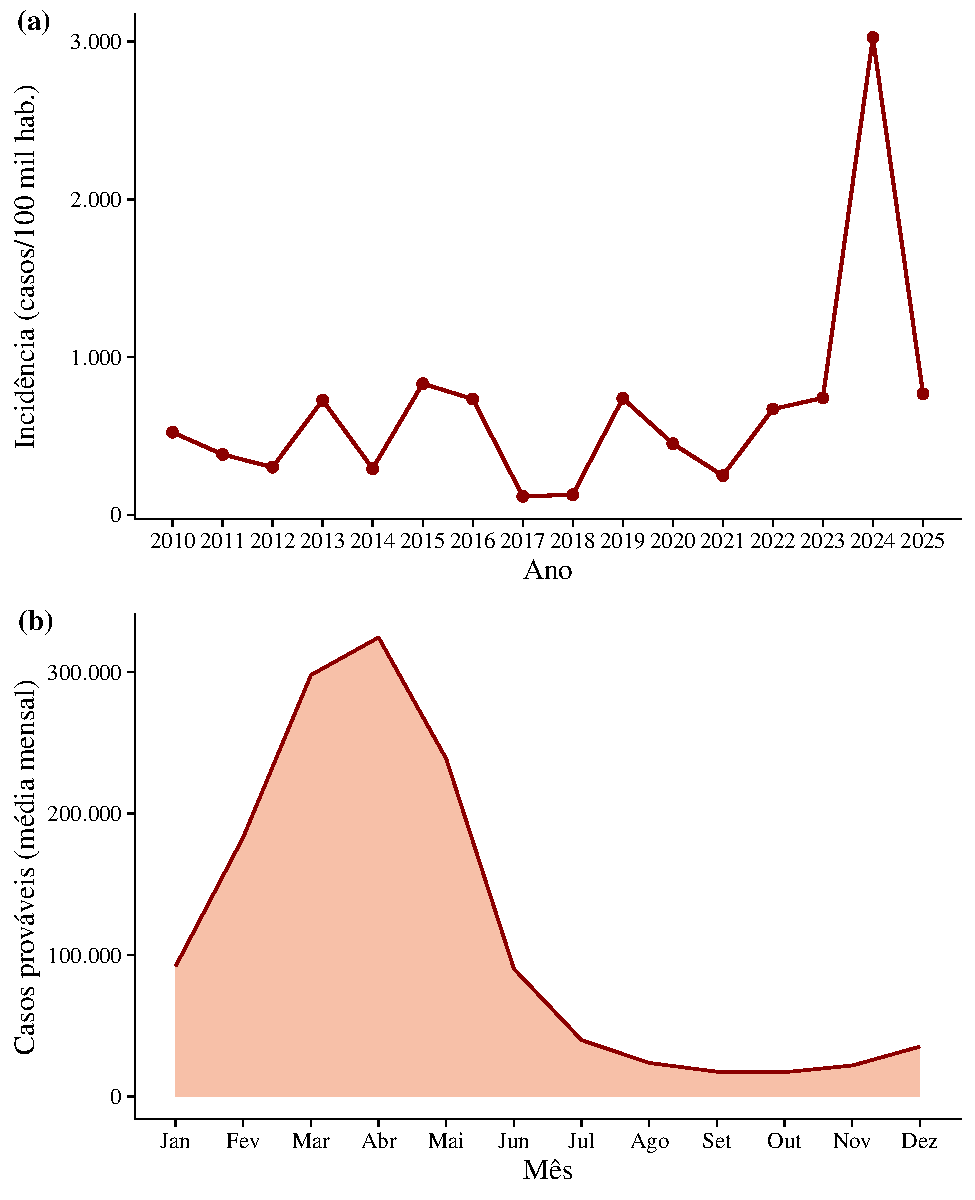
\includegraphics[width=0.91\textwidth,height=5.1cm,keepaspectratio,trim=0 288bp 0 0,clip]{fig_serie_temporal_dengue.pdf}
\par\medskip\raggedright Em 2024: \CasosDoisMilVinteQuatro{} casos e \TIDoisMilVinteQuatro{} por 100 mil habitantes; 29,1\% dos casos do painel.\fonte{SINAN e IBGE; elaboração do autor.}
\note{Leia a incidência por 100 mil habitantes. O pico de 2024 concentra quase três décimos da série acumulada. Em 2025 há recuo em relação a 2024, sem retorno automático aos menores níveis históricos.}
\end{frame}

\begin{frame}{Sazonalidade mensal}
\centering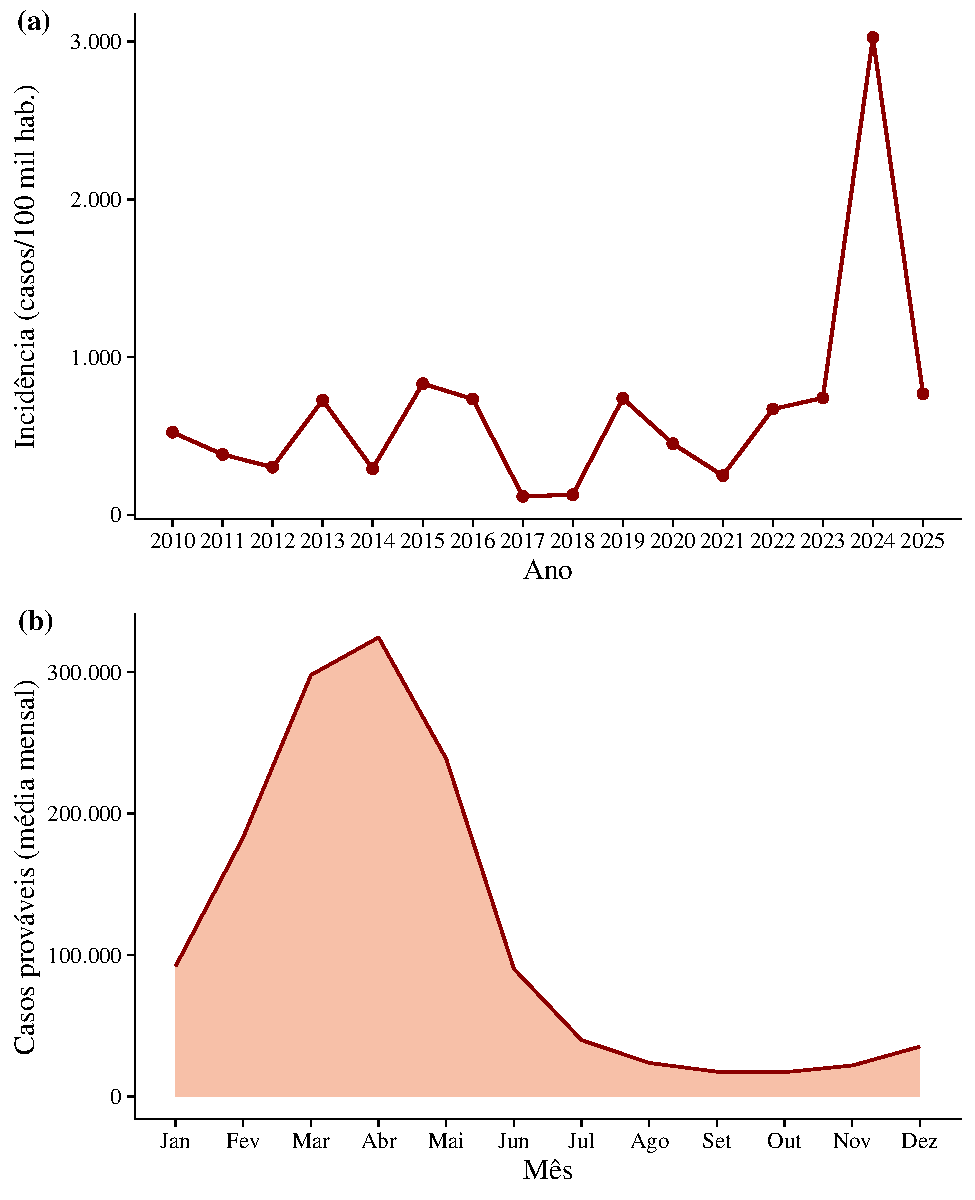
\includegraphics[width=0.91\textwidth,height=5.15cm,keepaspectratio,trim=0 0 0 288bp,clip]{fig_serie_temporal_dengue.pdf}\par\medskip\raggedright Maior concentração no primeiro semestre, com pico em abril.\fonte{SINAN; elaboração do autor.}
\note{Leia a média mensal do período. A agregação nacional pode ocultar calendários diferentes entre regiões.}
\end{frame}

\begin{frame}{Evolução regional da incidência}
\centering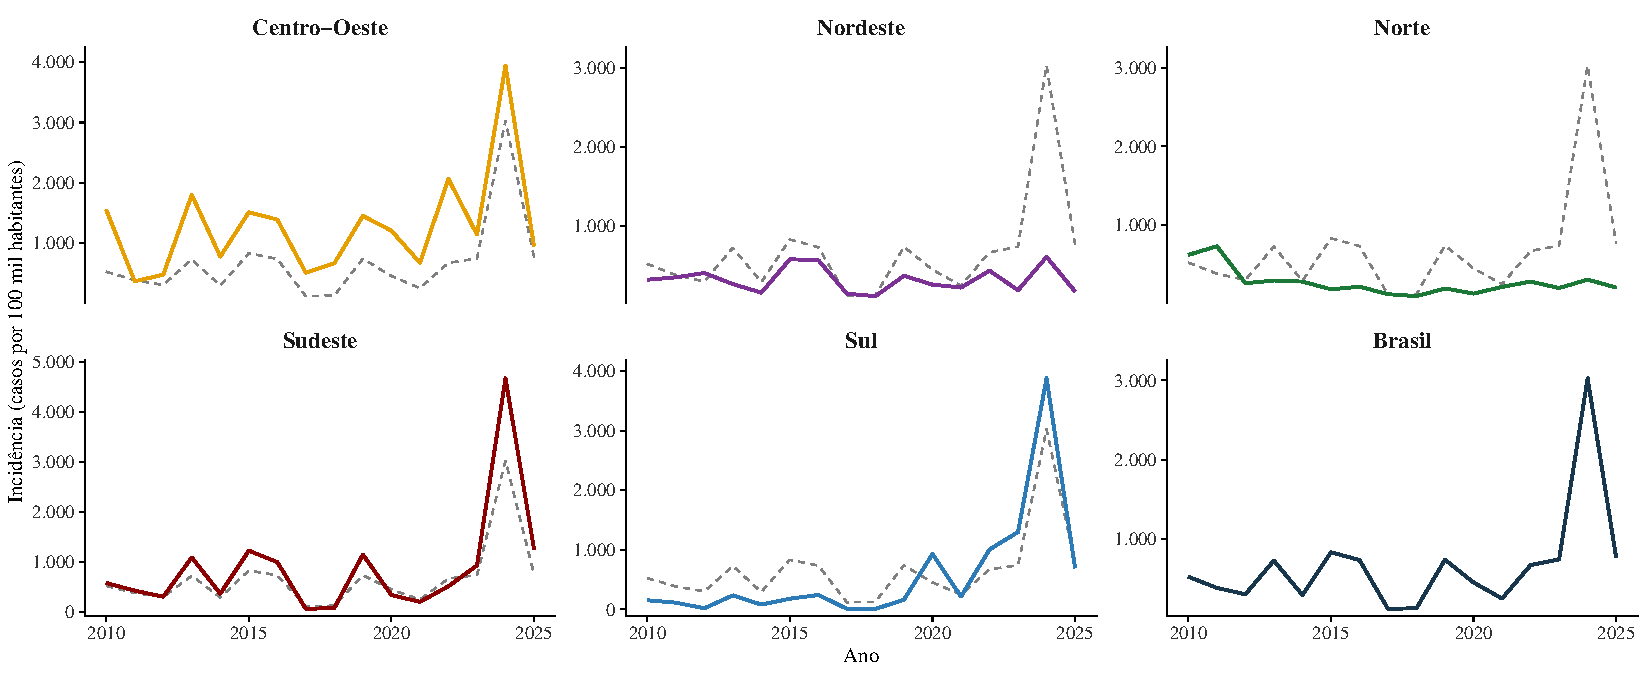
\includegraphics[width=0.98\textwidth,height=4.9cm,keepaspectratio]{fig_series_regioes_slides_2x3.pdf}
\par\medskip\raggedright A linha tracejada é a referência nacional. O último painel apresenta o Brasil; as escalas verticais variam entre painéis.\fonte{SINAN e IBGE; elaboração do autor.}
\note{Use o gráfico regional para distinguir trajetórias. Os cinco painéis regionais preservam os dados e as cores da monografia. A sexta posição apresenta a série nacional. Os eixos verticais mantêm escalas próprias, como na figura original; compare taxas pelos rótulos, e não apenas pela altura das curvas. Reserve explicações sobre clima e conectividade para a discussão.}
\end{frame}

\begin{frame}{Heatmap da incidência por UF e ano}
\centering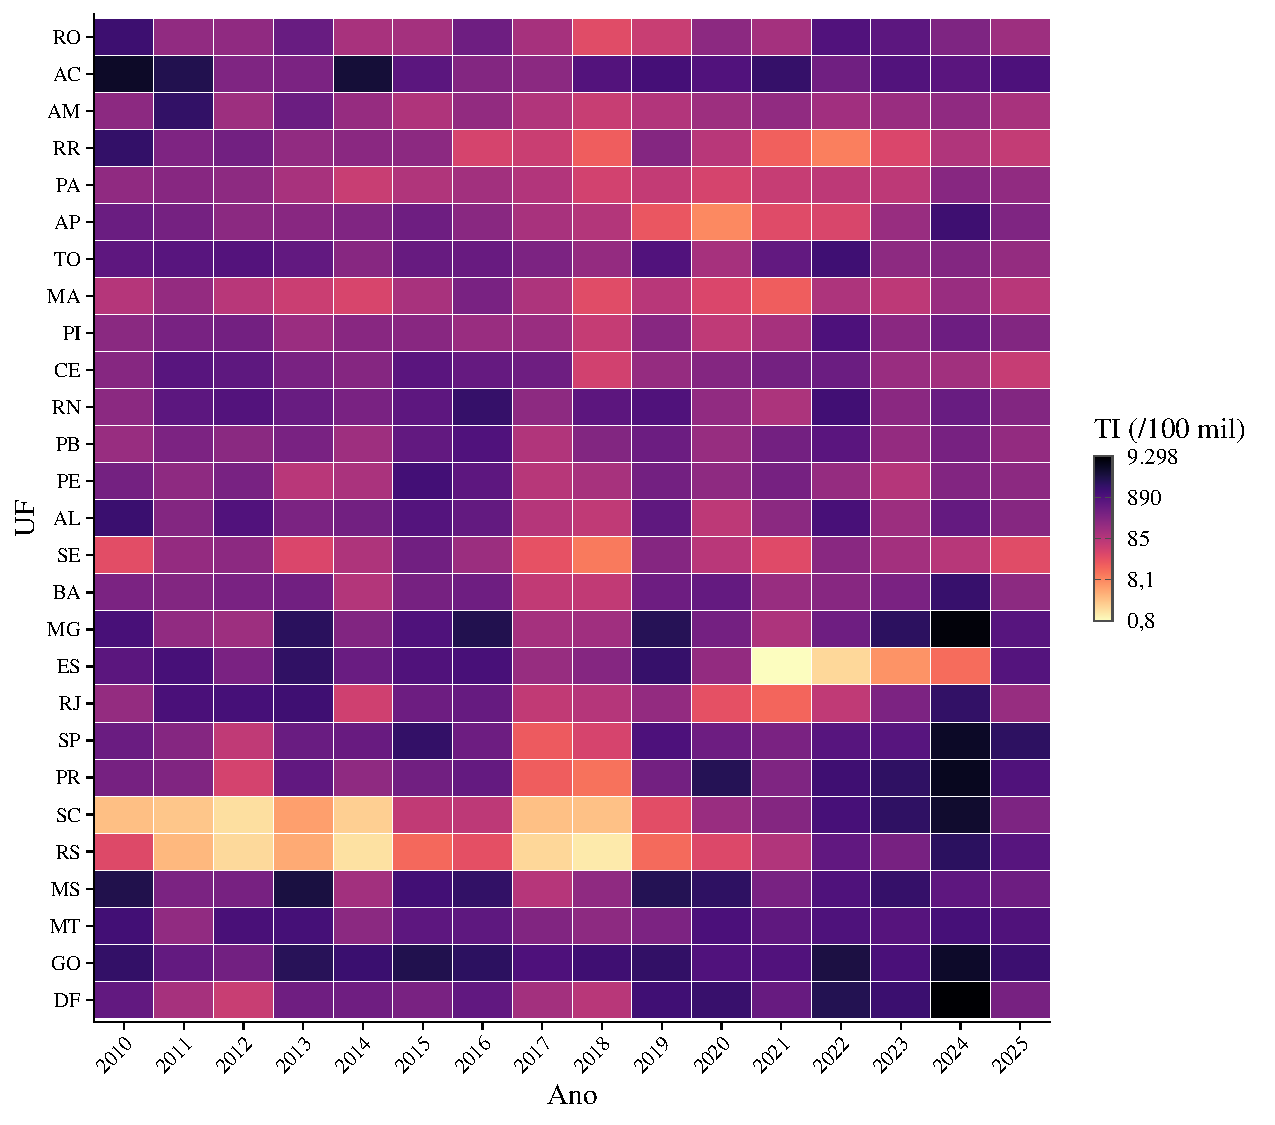
\includegraphics[width=0.95\textwidth,height=6cm,keepaspectratio]{fig_heatmap_incidencia_uf_ano.pdf}\fonte{SINAN e IBGE; escala logarítmica da incidência.}
\note{O logaritmo permite visualizar ordens de grandeza sem a cor ser dominada por poucas UFs e anos. Leia o valor pelas classes da legenda, e não como diferenças lineares de cor.}
\end{frame}



\begin{frame}{Carga acumulada municipal}
\begin{columns}[c]\begin{column}{0.61\textwidth}\centering
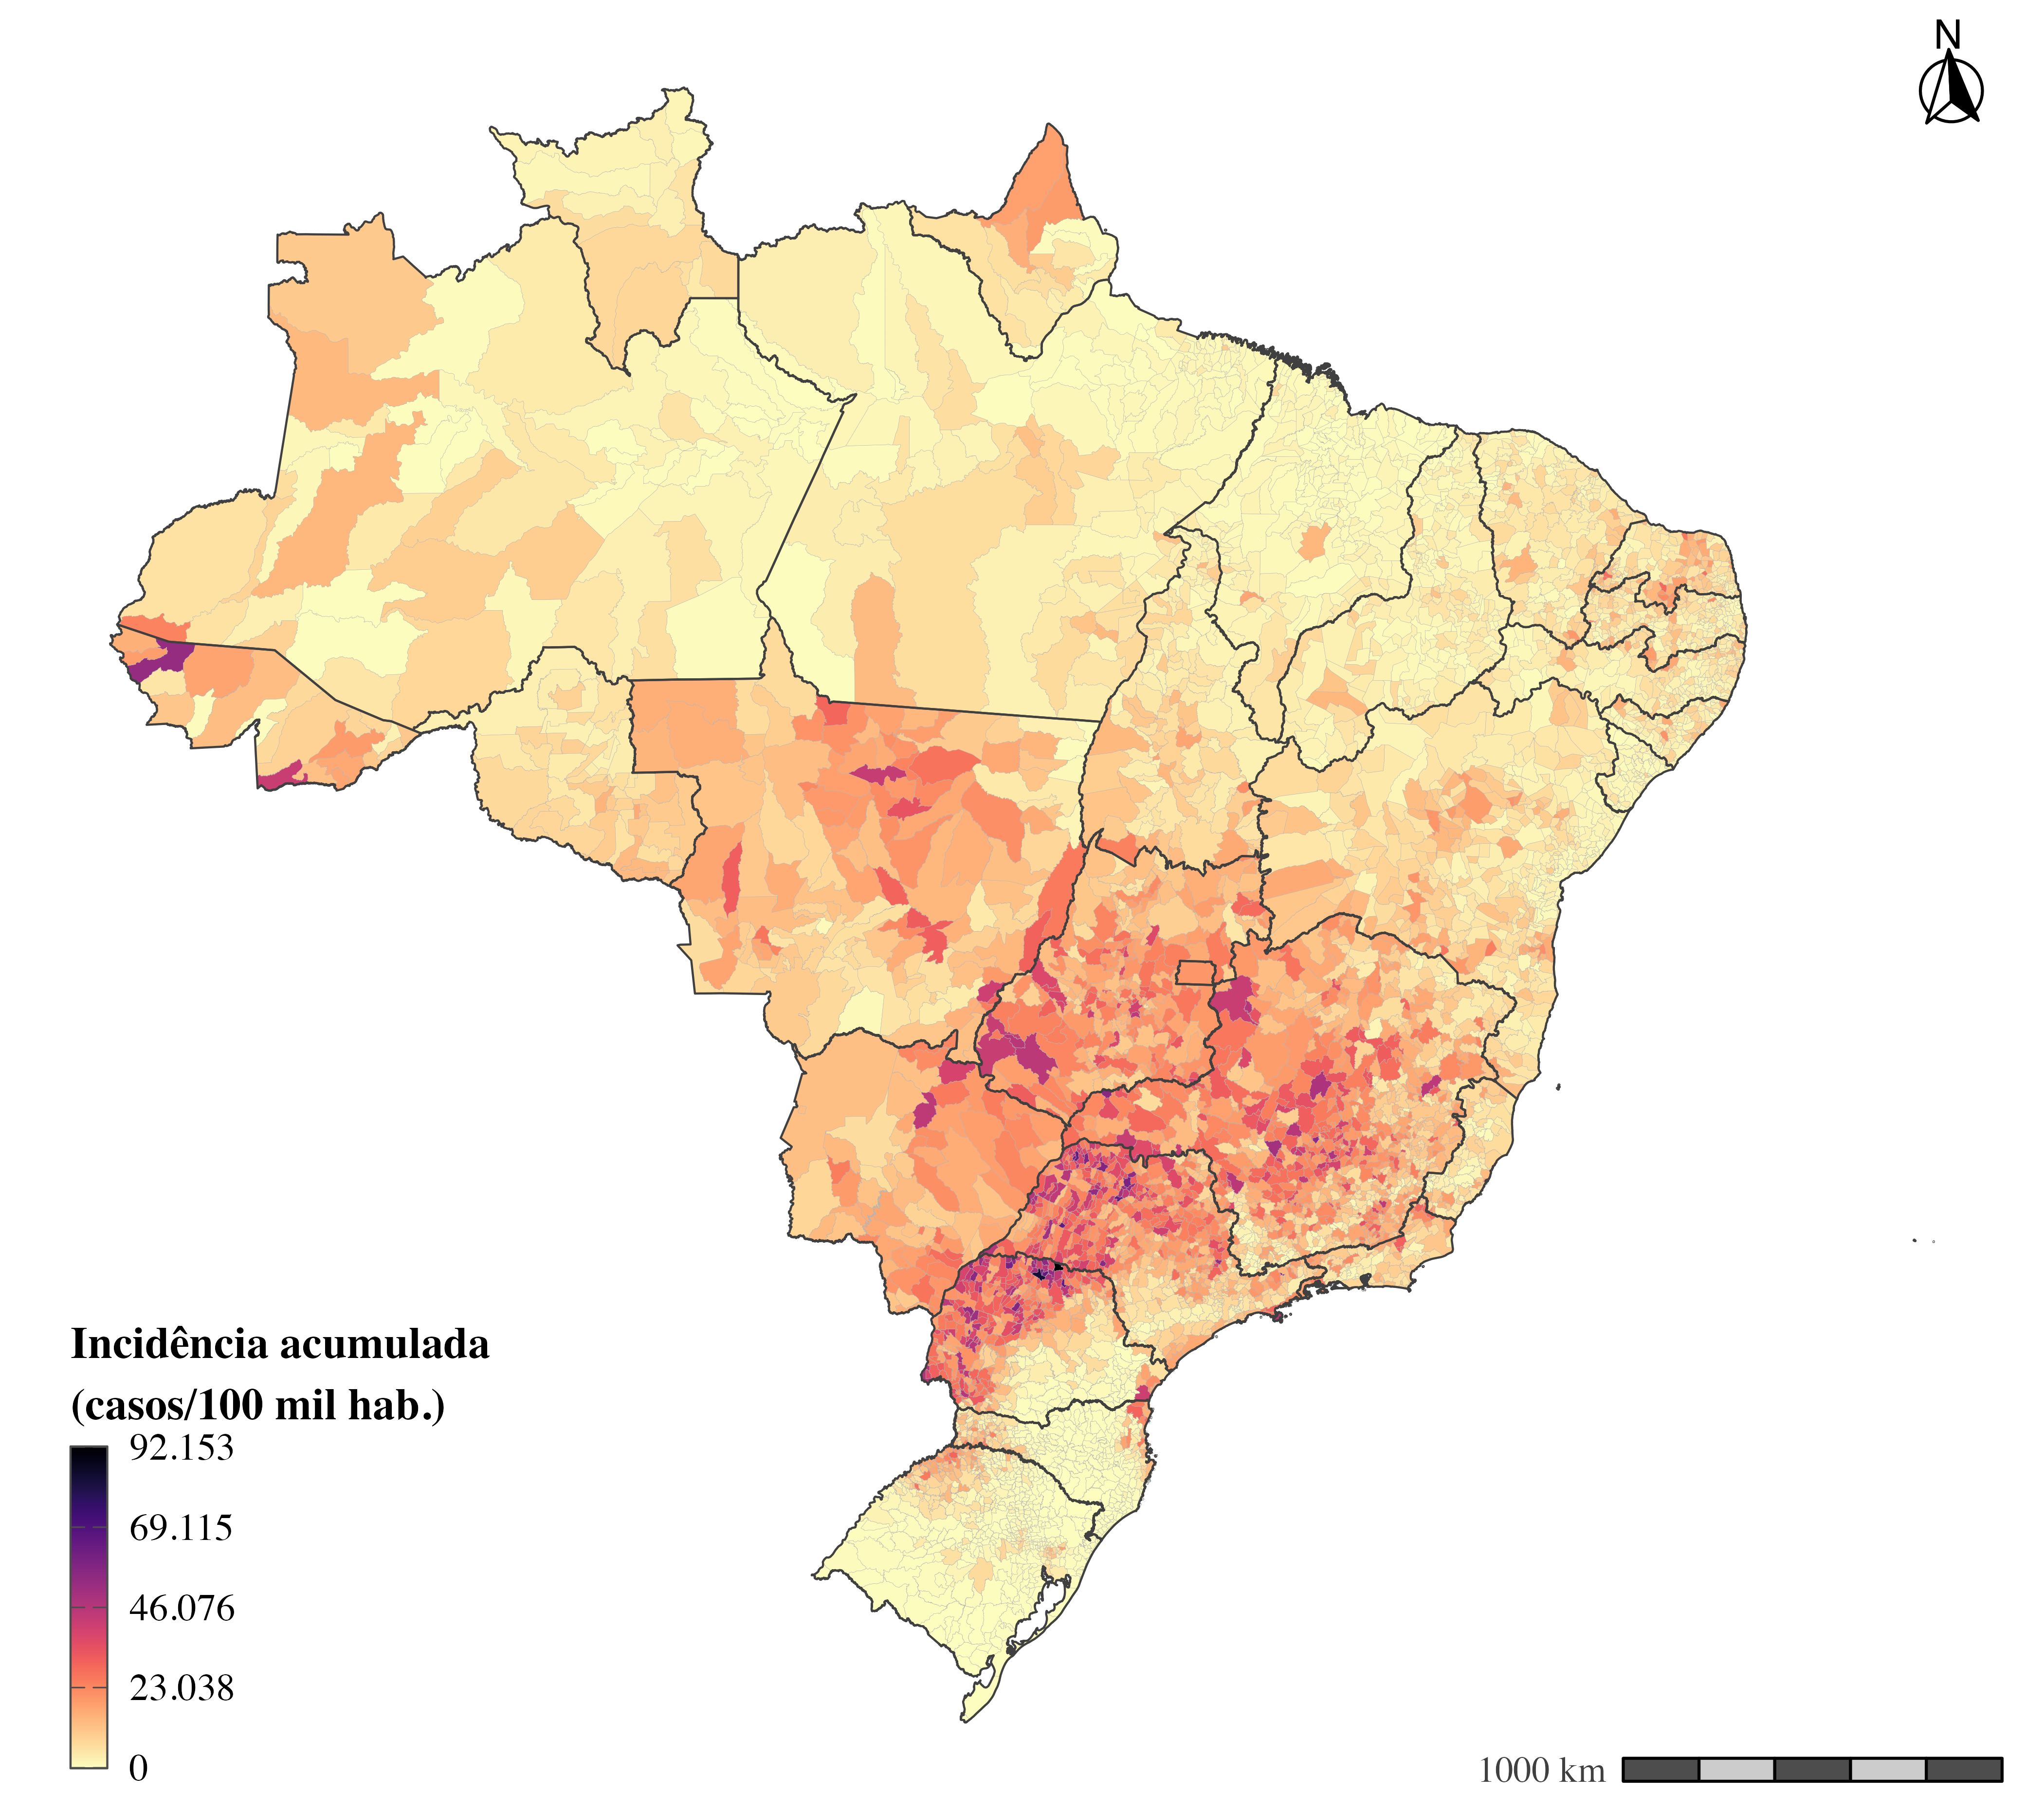
\includegraphics[width=\linewidth,height=6.15cm,keepaspectratio]{fig_mapa_incidencia_acumulada.png}
\end{column}\begin{column}{0.36\textwidth}Razão de casos acumulados por população média.
\medskip
Contrastes municipais concentrados sobretudo no Centro-Sul.
\medskip
A legenda usa a escala do período completo, por 100 mil habitantes.\end{column}\end{columns}\fonte{SINAN e IBGE; elaboração do autor.}
\note{Leia o denominador antes das cores. Não interprete a razão como taxa anual nem como percentual de pessoas que tiveram dengue. O mapa motiva a investigação da associação espacial.}
\end{frame}

\begin{frame}{Recorrência de anos epidêmicos}
\begin{columns}[c]\begin{column}{0.61\textwidth}\centering
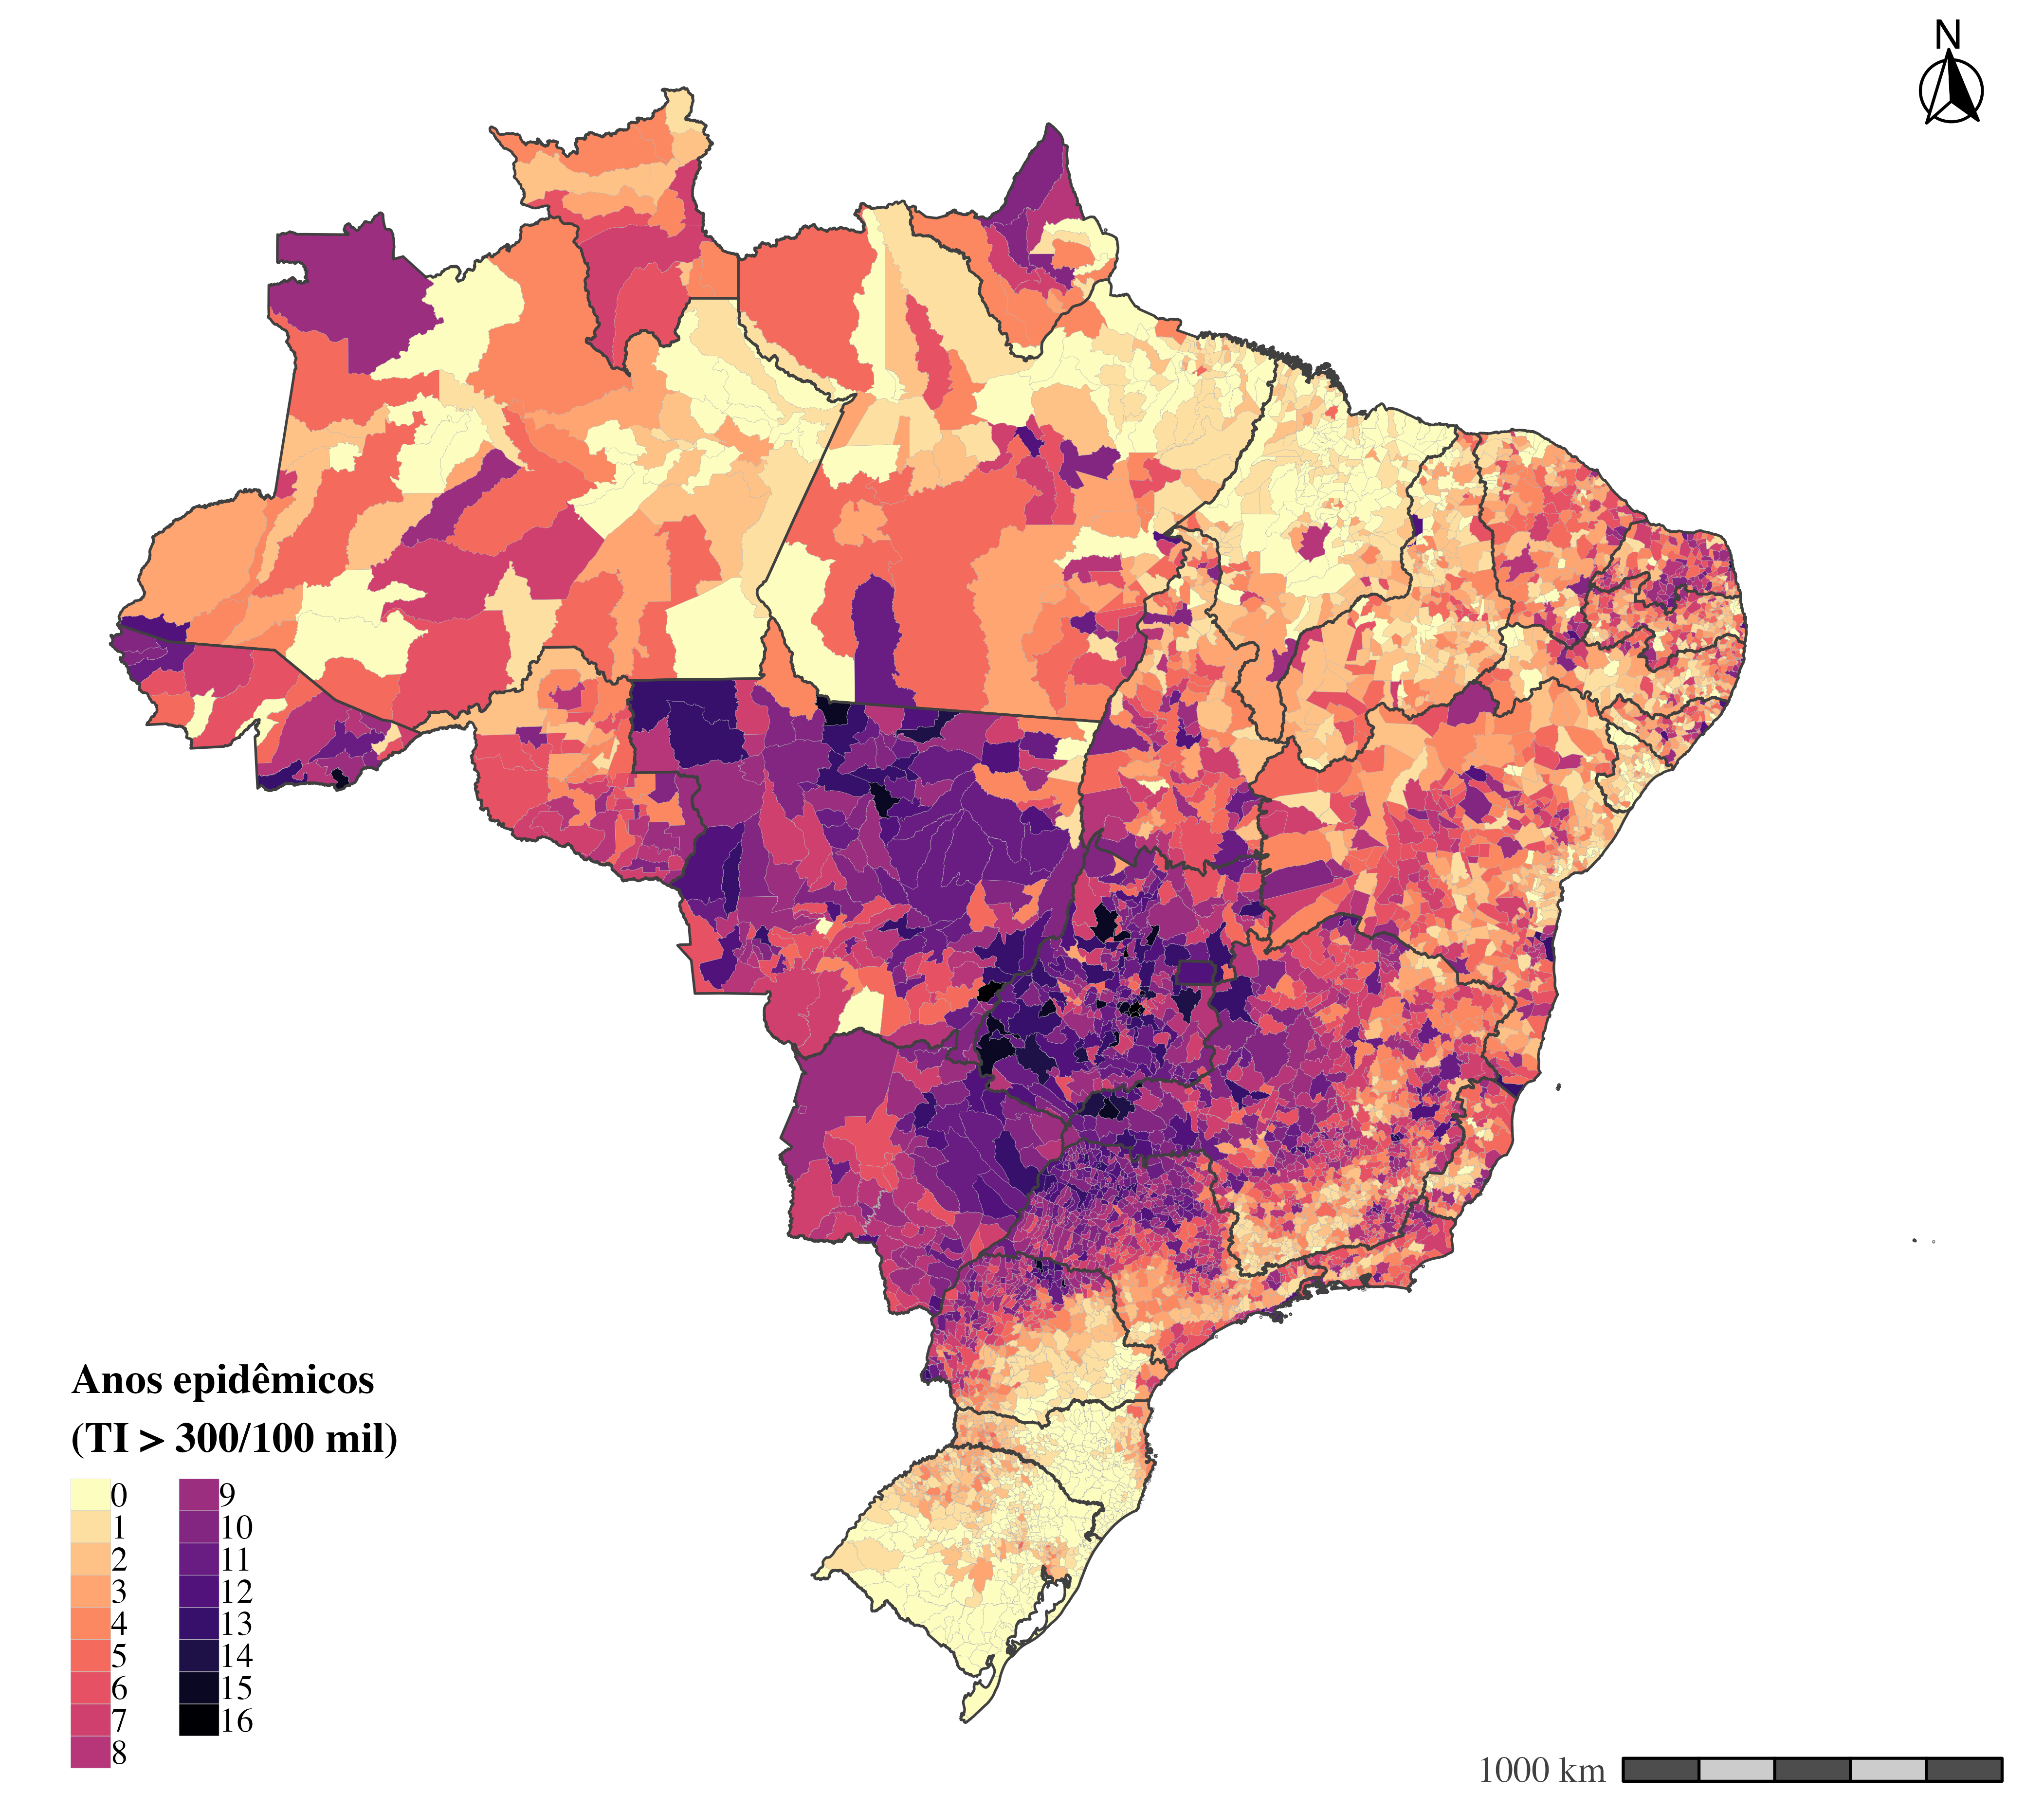
\includegraphics[width=\linewidth,height=6.15cm,keepaspectratio]{fig_mapa_persistencia_epidemica.png}
\end{column}\begin{column}{0.36\textwidth}\[H_i=\sum_{t=2010}^{2025}\mathbf1(TI_{it}>300)\]
\PctMunPersistencia{} dos municípios tiveram pelo menos dez anos acima do limiar.
\medskip
A contagem não implica transmissão contínua nos mesmos indivíduos.\end{column}\end{columns}\fonte{SINAN e IBGE; elaboração do autor.}
\note{Este mapa conta anos. Diferencie-o da contagem das oito formulações. O limiar de 300 é descritivo e não foi usado para selecionar as zonas da varredura.}
\end{frame}



\begin{frame}{Autocorrelação espacial nos 16 anos}
\centering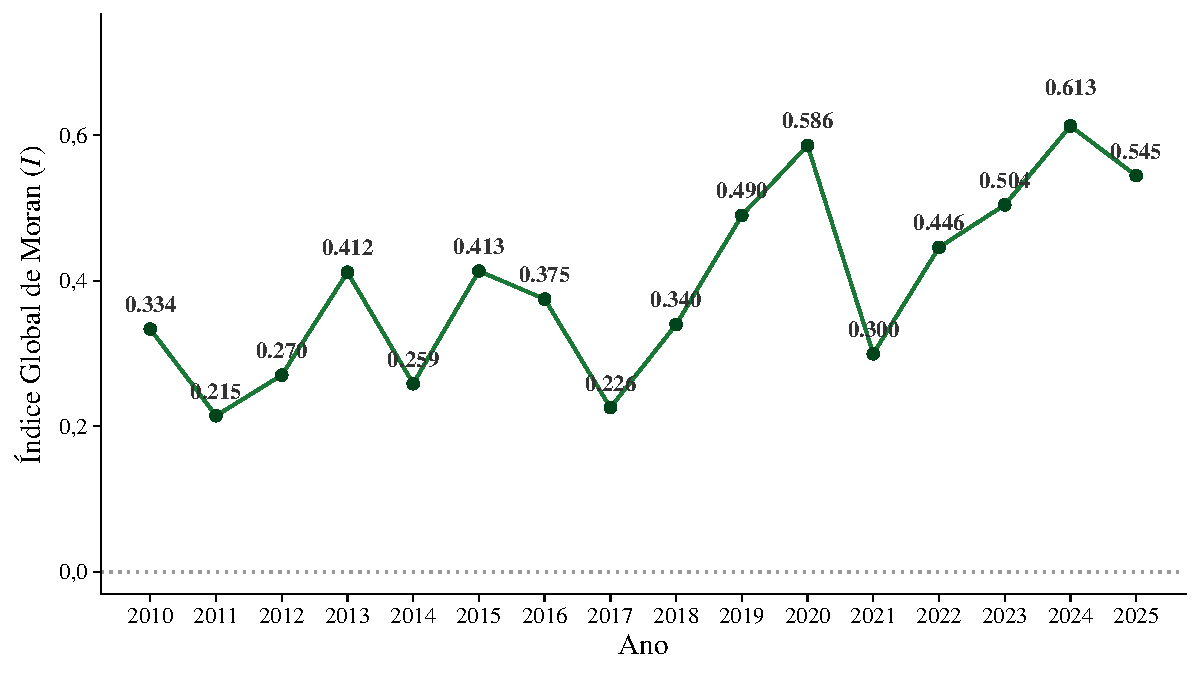
\includegraphics[width=0.92\textwidth,height=4.9cm,keepaspectratio]{fig_evolucao_moran.pdf}
\par\medskip\raggedright Moran positivo e significativo a 5\% em todos os anos: \MoranMin{} a \MoranMax{}, com máximo em 2024.\fonte{SINAN e IBGE; elaboração do autor.}
\note{A associação espacial acompanha os anos de incidência de forma variável. Não confunda índice alto com incidência alta: um descreve a organização espacial, o outro a magnitude.}
\end{frame}

\begin{frame}{Associação espacial local}
\begin{columns}[c]\begin{column}{0.61\textwidth}\centering
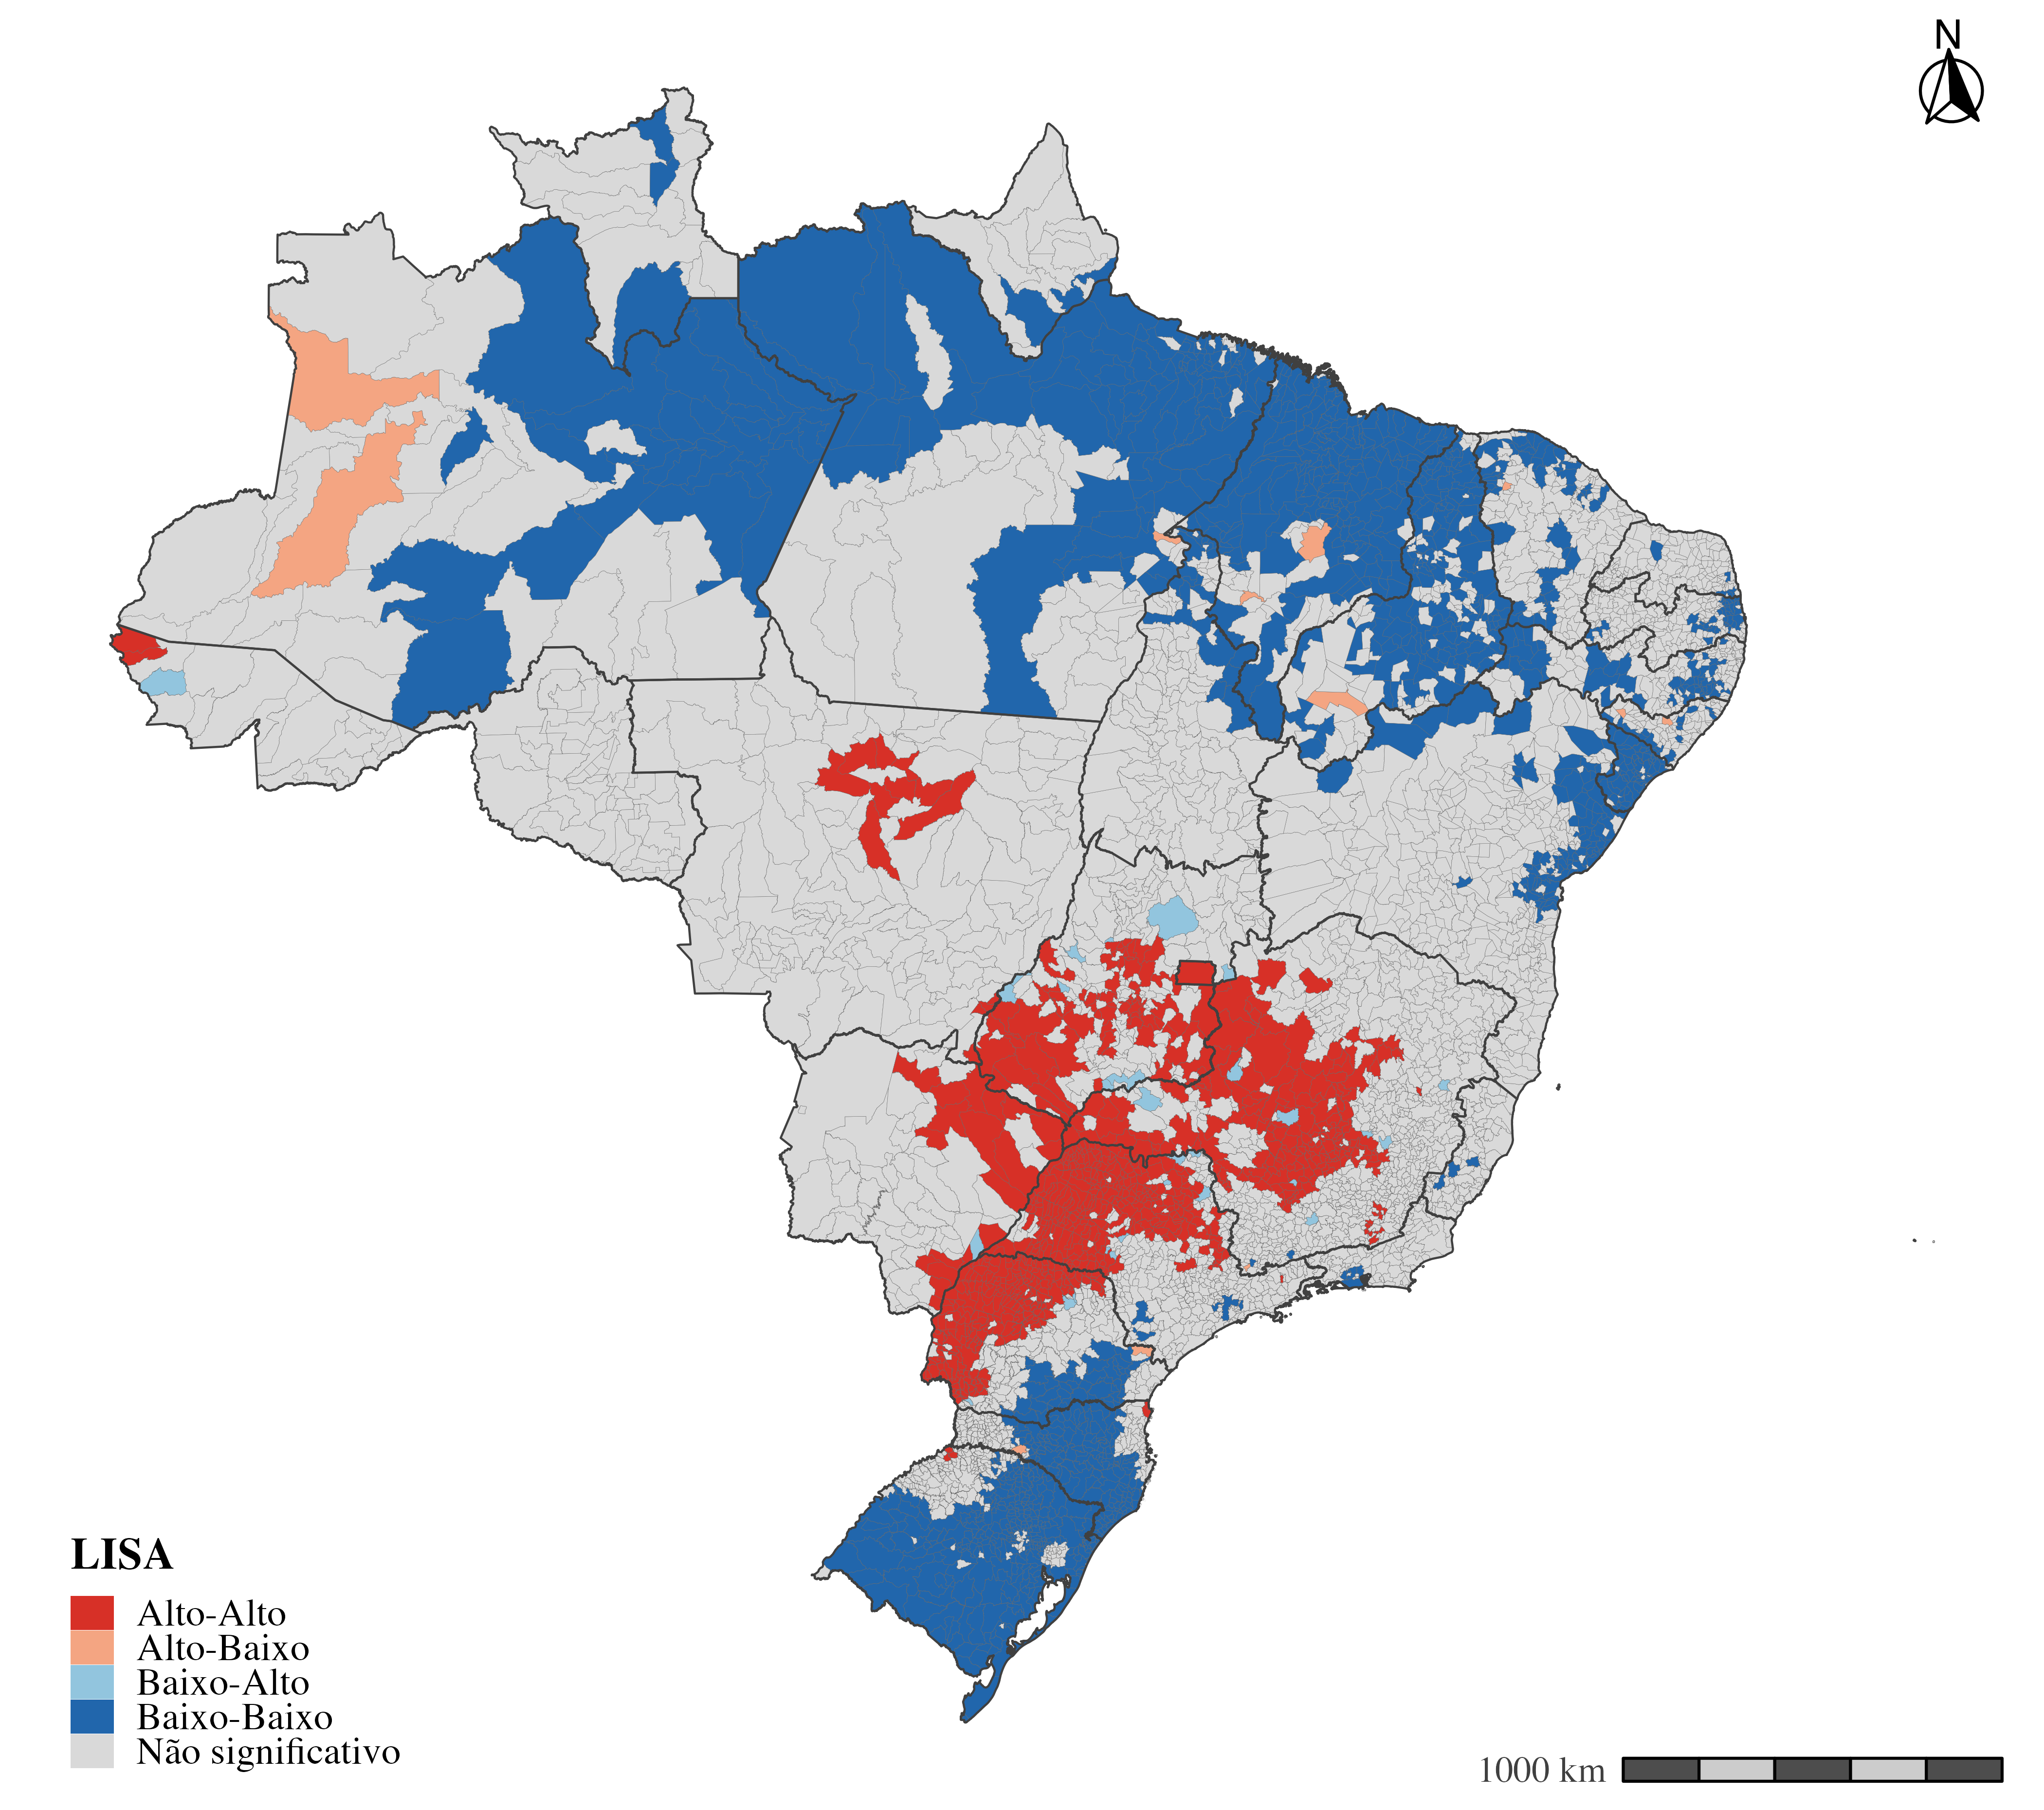
\includegraphics[width=\linewidth,height=6.15cm,keepaspectratio]{fig_mapa_lisa.png}
\end{column}\begin{column}{0.36\textwidth}\LisaHH{} municípios alto-alto; \LisaLL{} baixo-baixo.
\medskip
\LisaHL{} alto-baixo e \LisaLH{} baixo-alto.
\medskip
\LisaNS{} sem significância nominal.
\medskip
\small Leitura exploratória, sem correção de multiplicidade local.\end{column}\end{columns}\fonte{SINAN e IBGE; elaboração do autor.}
\note{Alto-alto e baixo-baixo têm associação positiva. A ausência de significância não significa ausência de dengue. Aqui a referência é a média da razão acumulada entre municípios, distinta da referência populacional da varredura.}
\end{frame}

\begin{frame}{Incidência por estratos das covariáveis}
\small
\begin{tabularx}{\textwidth}{@{}Xrrr@{}}\toprule
Indicador & Nível 1 & Nível 2 & Nível 3\\\midrule
Calor & 431,7 & 738,3 & 1.088,7\\
Esgoto & 797,6 & 483,5 & 357,5\\
Densidade urbana & 613,1 & 768,4 & 649,2\\
Proporção urbana & 436,5 & 558,3 & 732,8\\
Água & 821,7 & 502,5 & 311,7\\
Lixo & 779,0 & 526,8 & 305,5\\
Índice composto & 789,5 & 602,5 & 330,2\\
\bottomrule\end{tabularx}\par\vspace{0.25cm}\noindent\normalsize Casos por 100 mil pessoas-ano em 2010--2025.
\medskip Níveis de saneamento ordenados da maior para a menor cobertura; demais indicadores, do menor para o maior valor.
\fonte{Tabela de incidência por tercis; SINAN, IBGE, ERA5-Land e MapBiomas.}
\note{As taxas agregam casos e pessoas-ano de todos os municípios do estrato. Os níveis têm números semelhantes de municípios, mas populações e composições regionais distintas. A taxa mais alta em grupos com maior cobertura de saneamento não identifica um efeito prejudicial do saneamento. A comparação é descritiva e pode refletir composição territorial e diferenças de notificação.}
\end{frame}


\begin{frame}{Zonas de alto risco sem ajuste}
\begin{columns}[c]\begin{column}{0.61\textwidth}\centering
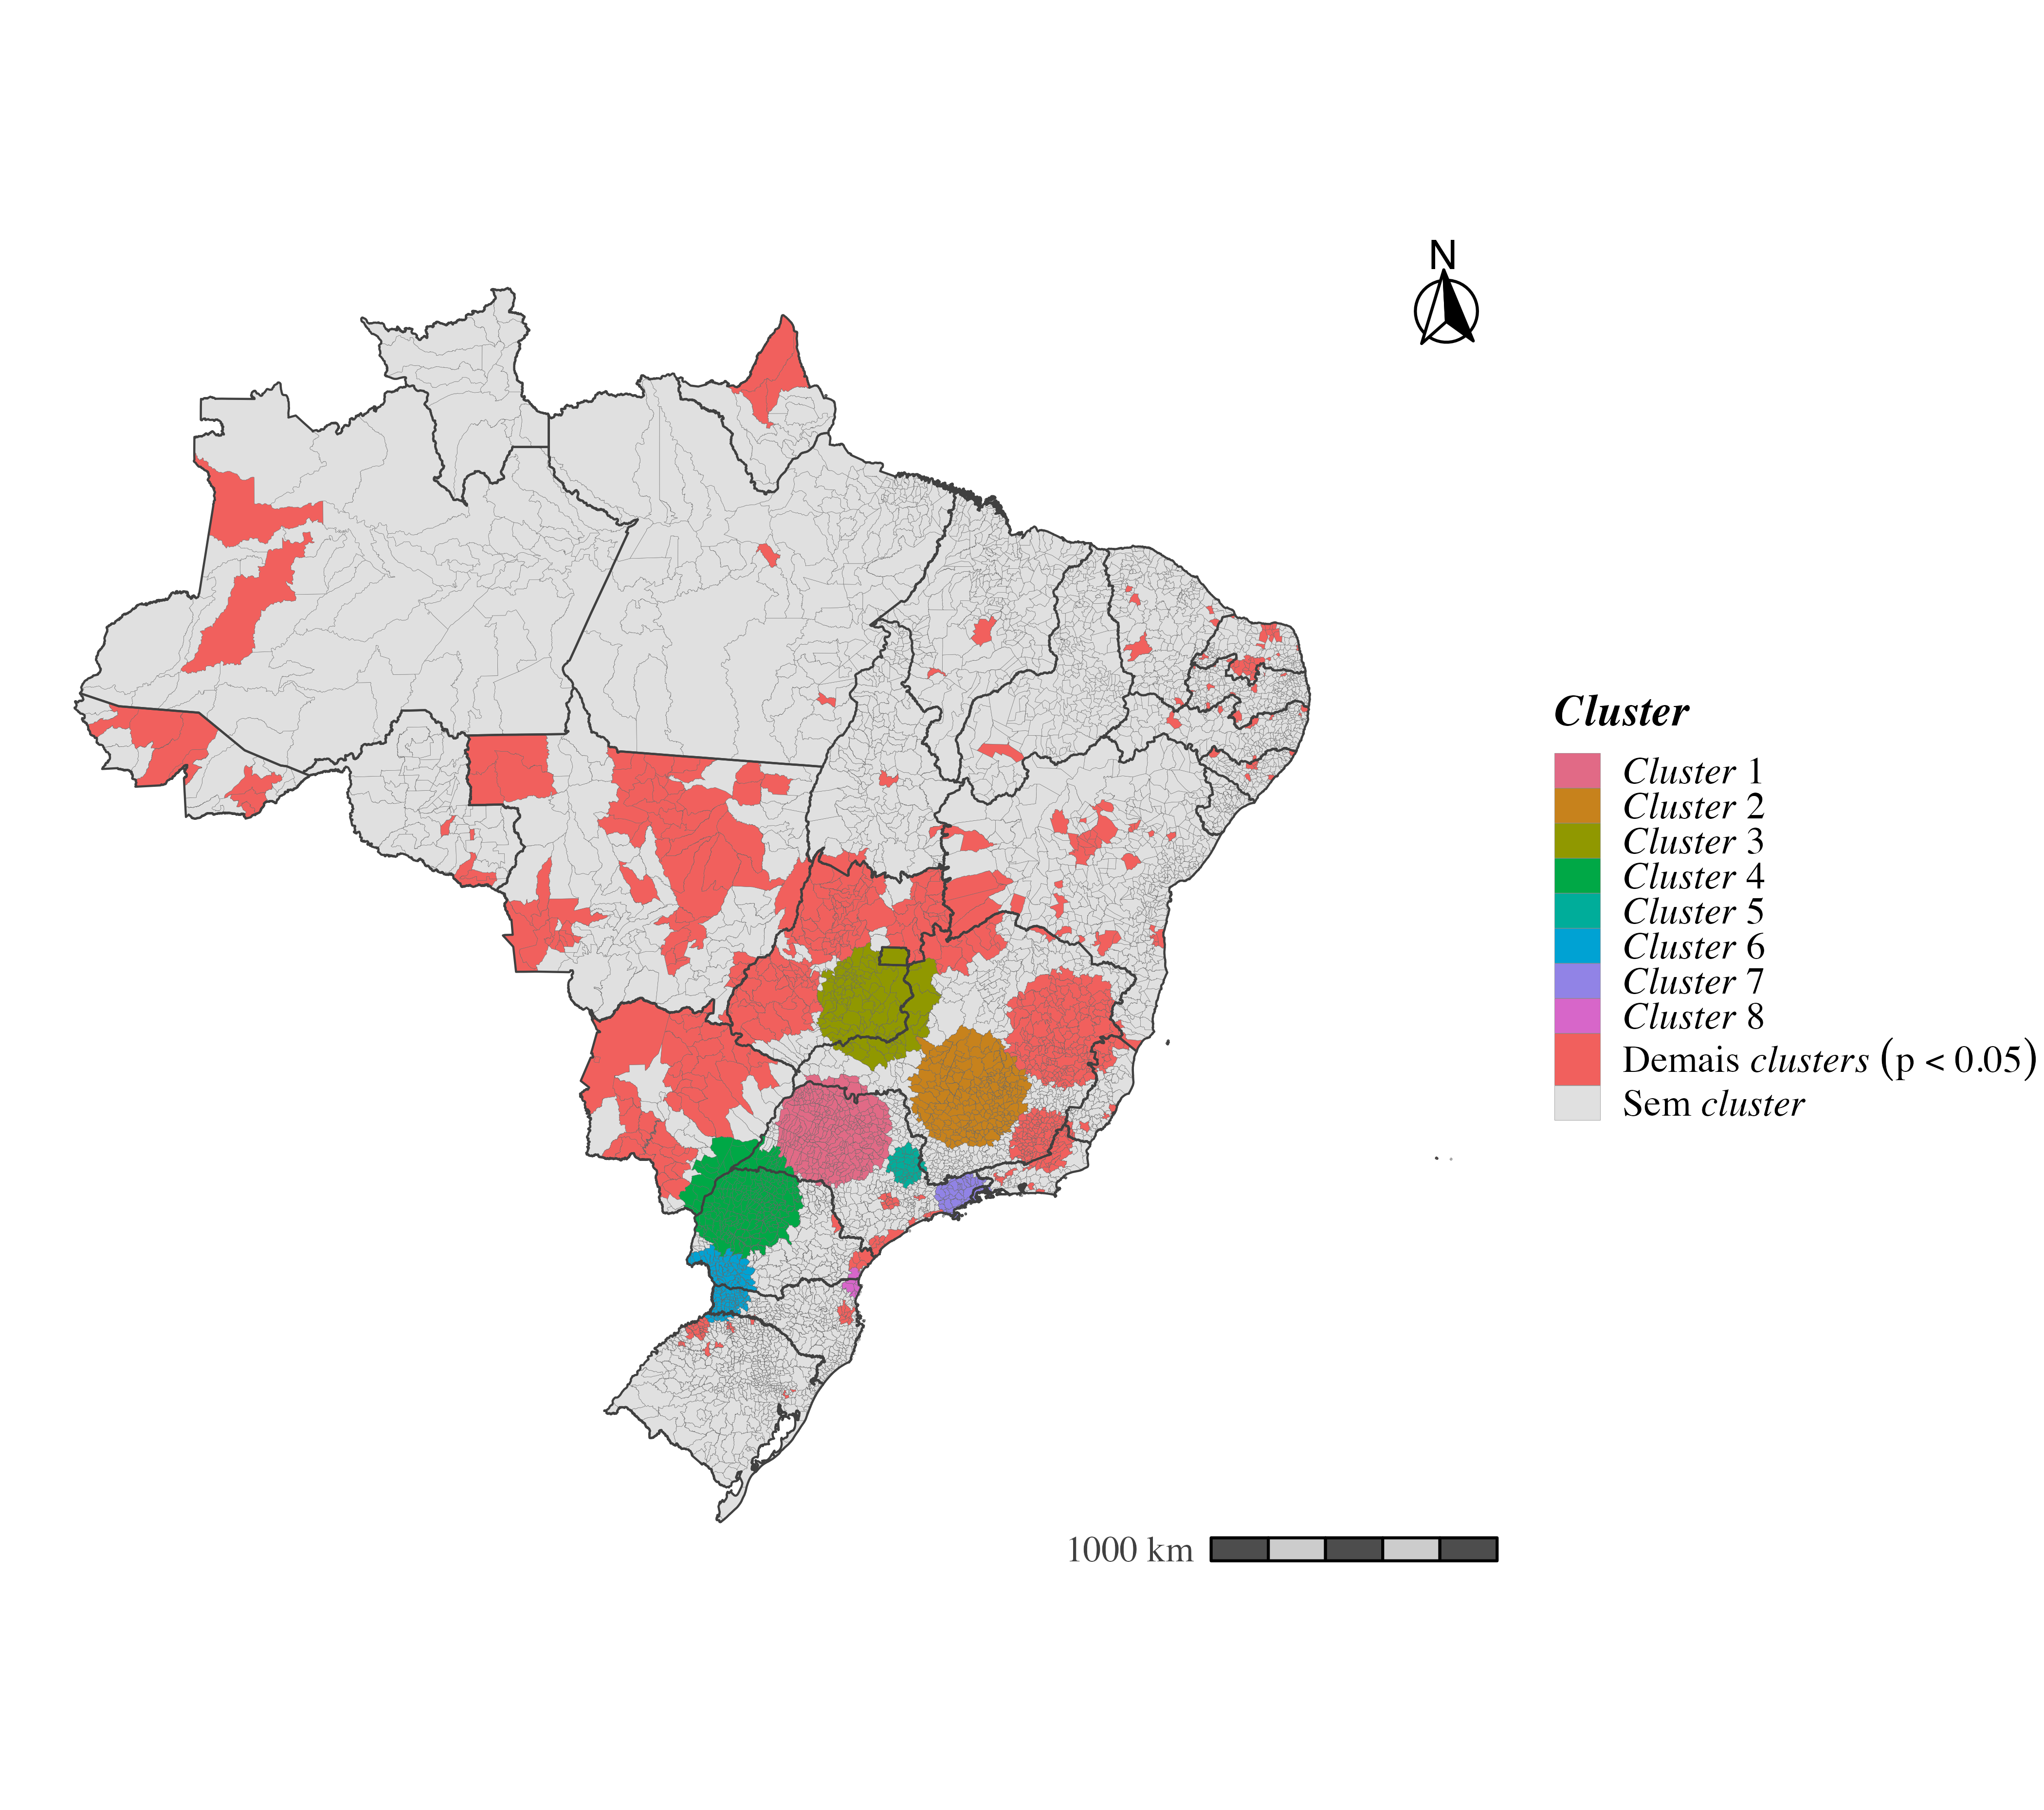
\includegraphics[width=\linewidth,height=6.15cm,keepaspectratio]{fig_mapa_clusters_satscan_puro.png}
\end{column}\begin{column}{0.36\textwidth}\ScanNumClusters{} zonas significativas.
\medskip
\ScanCobMunicipios{} municípios (\ScanCobMunicipiosPct{}).
\medskip
\ScanCobCasosPct{} dos casos em \ScanCobPopPct{} da população.
\medskip
\small Reporte sem sobreposição; nível de 5\%.\end{column}\end{columns}\fonte{SINAN e IBGE; elaboração do autor.}
\note{A fração dos casos é maior que a participação populacional das zonas. O mapa diferencia as principais zonas e as demais significativas. O centro da janela não deve ser tratado como origem da transmissão.}
\end{frame}

\begin{frame}{Zona primária: Adolfo (SP)}
\begin{tabularx}{\textwidth}{@{}Xr@{}}\toprule
Municípios na zona & \ScanPrimMunicipios{}\\
Raio da janela & \ScanPrimRaioKm{} km\\
Casos observados & \ScanPrimCasosObs{}\\
Casos esperados & \ScanPrimCasosEsp{}\\
Risco relativo & \ScanPrimRR{}\\\bottomrule
\end{tabularx}\par\vspace{0.25cm}\noindent Adolfo é o centro da janela de maior verossimilhança.
\medskip O RR compara a zona inteira ao seu exterior.
%\fonte{Relatório e auditoria da varredura sem ajuste.}
\note{Retome os métodos usando um resultado real. Dividir observado por esperado não fornece exatamente 2,99, pois o RR inclui o contraste externo. O centro não representa sozinho os 319 municípios.}
\end{frame}

\begin{frame}{Comparação das oito formulações}
\small
\begin{tabularx}{\textwidth}{@{}Xrlrr@{}}\toprule
Formulação & Zonas & Polo primário & RR & WMAPE (\%)\\\midrule
Sem ajuste &129&Adolfo (SP)&2,99&75,1\\
Calor &128&Queluzito (MG)&2,08&64,9\\
Esgoto &178&Iacri (SP)&2,79&71,9\\
Densidade urbana &136&Araújos (MG)&2,73&74,3\\
Proporção urbana &158&Iacri (SP)&3,11&74,4\\
Água &193&Iacri (SP)&2,70&70,5\\
Lixo &195&Iacri (SP)&2,86&72,1\\
Índice composto &184&Araújos (MG)&2,58&71,9\\\bottomrule
\end{tabularx}\par\vspace{0.25cm}\noindent\normalsize Sob calor, o WMAPE cai 10,2 pontos percentuais e permanecem 128 zonas.
%\fonte{Tabela comparativa do manuscrito; consolidação das oito rodadas.}
\note{Destaque que o número de zonas pode subir após um ajuste: a mudança dos esperados pode fragmentar zonas ou detectar outros excessos. O ajuste por calor foi destacado por reduzir mais o WMAPE preservando uma coleção extensa, sem validação preditiva.}
\end{frame}

\begin{frame}{Zonas após padronização por calor}
\begin{columns}[c]\begin{column}{0.61\textwidth}\centering
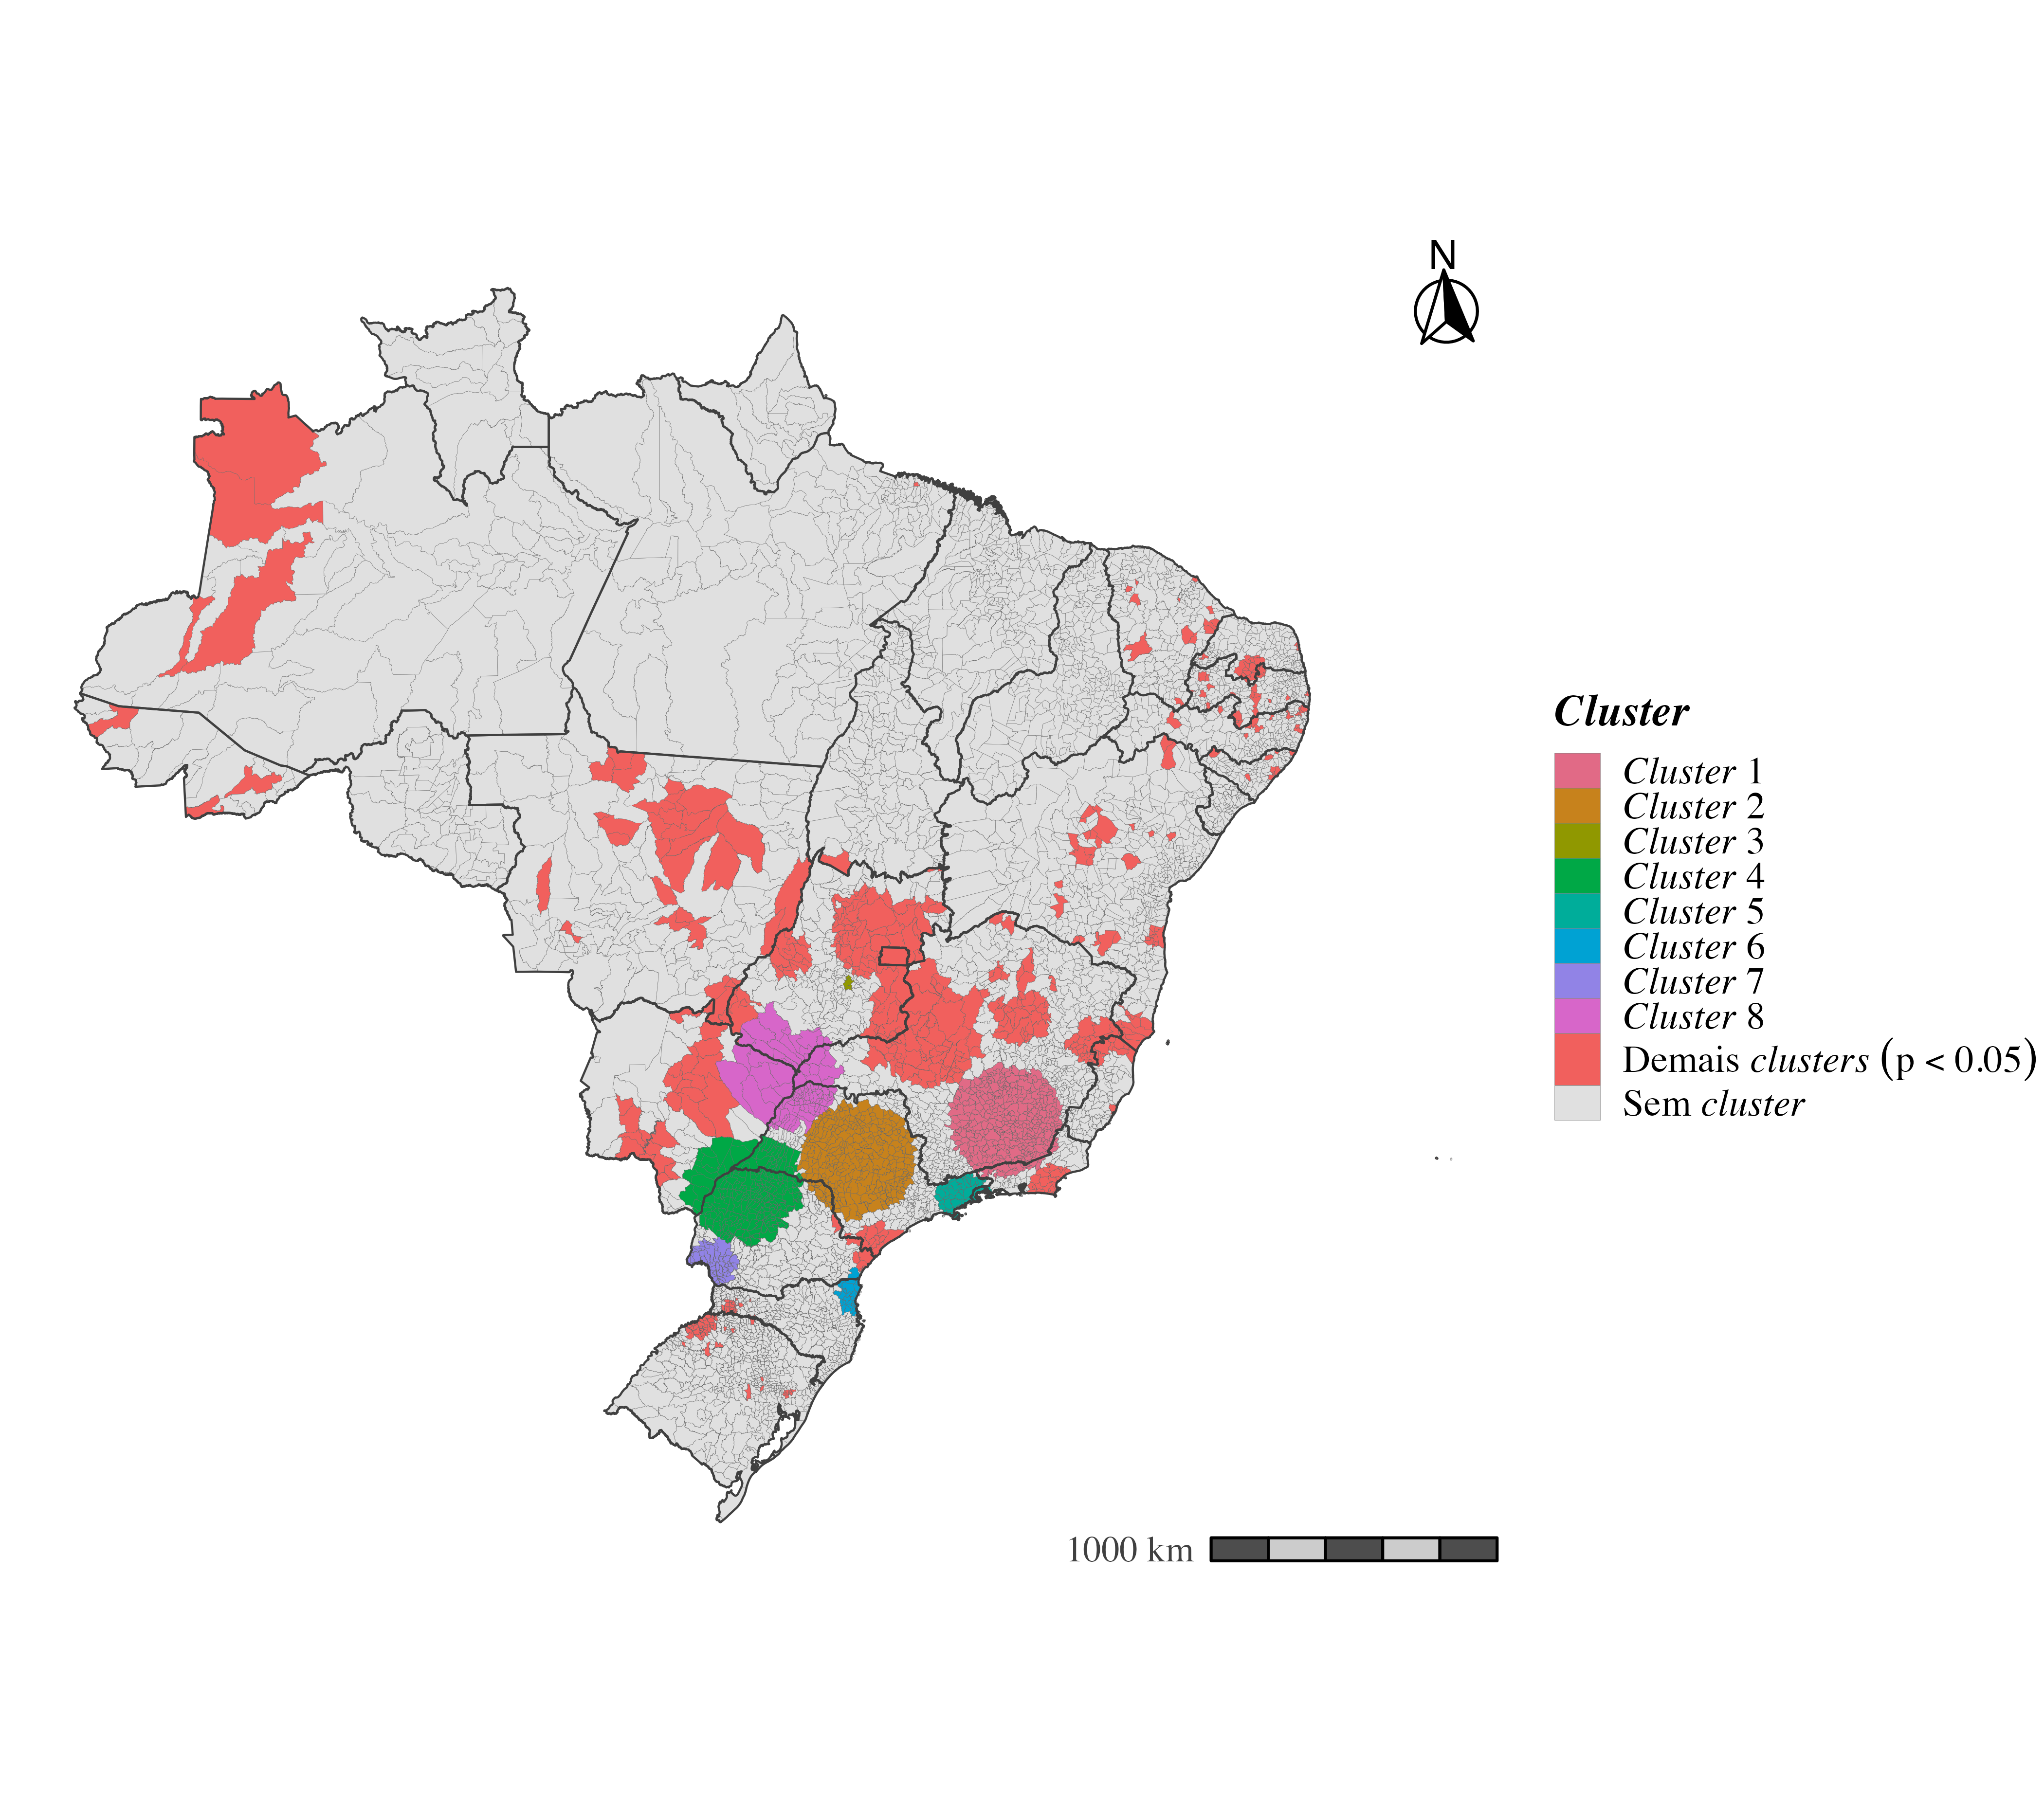
\includegraphics[width=\linewidth,height=6.15cm,keepaspectratio]{fig_mapa_clusters_satscan_termica.png}
\end{column}\begin{column}{0.36\textwidth}128 zonas; 63,3\% dos casos.
\medskip
Primário: Queluzito (MG), com 362 municípios e RR de 2,08.
\medskip
Jaccard de 56\% com a coleção sem ajuste.\end{column}\end{columns}\fonte{SINAN e IBGE; elaboração do autor.}
\note{A contagem de zonas quase não muda, mas a composição municipal muda bastante. Os primários são zonas diferentes; comparar RR 2,99 e 2,08 não estima uma redução do risco nos mesmos municípios.}
\end{frame}

\begin{frame}{Risco relativo municipal sem ajuste}
\begin{columns}[c]\begin{column}{0.61\textwidth}\centering
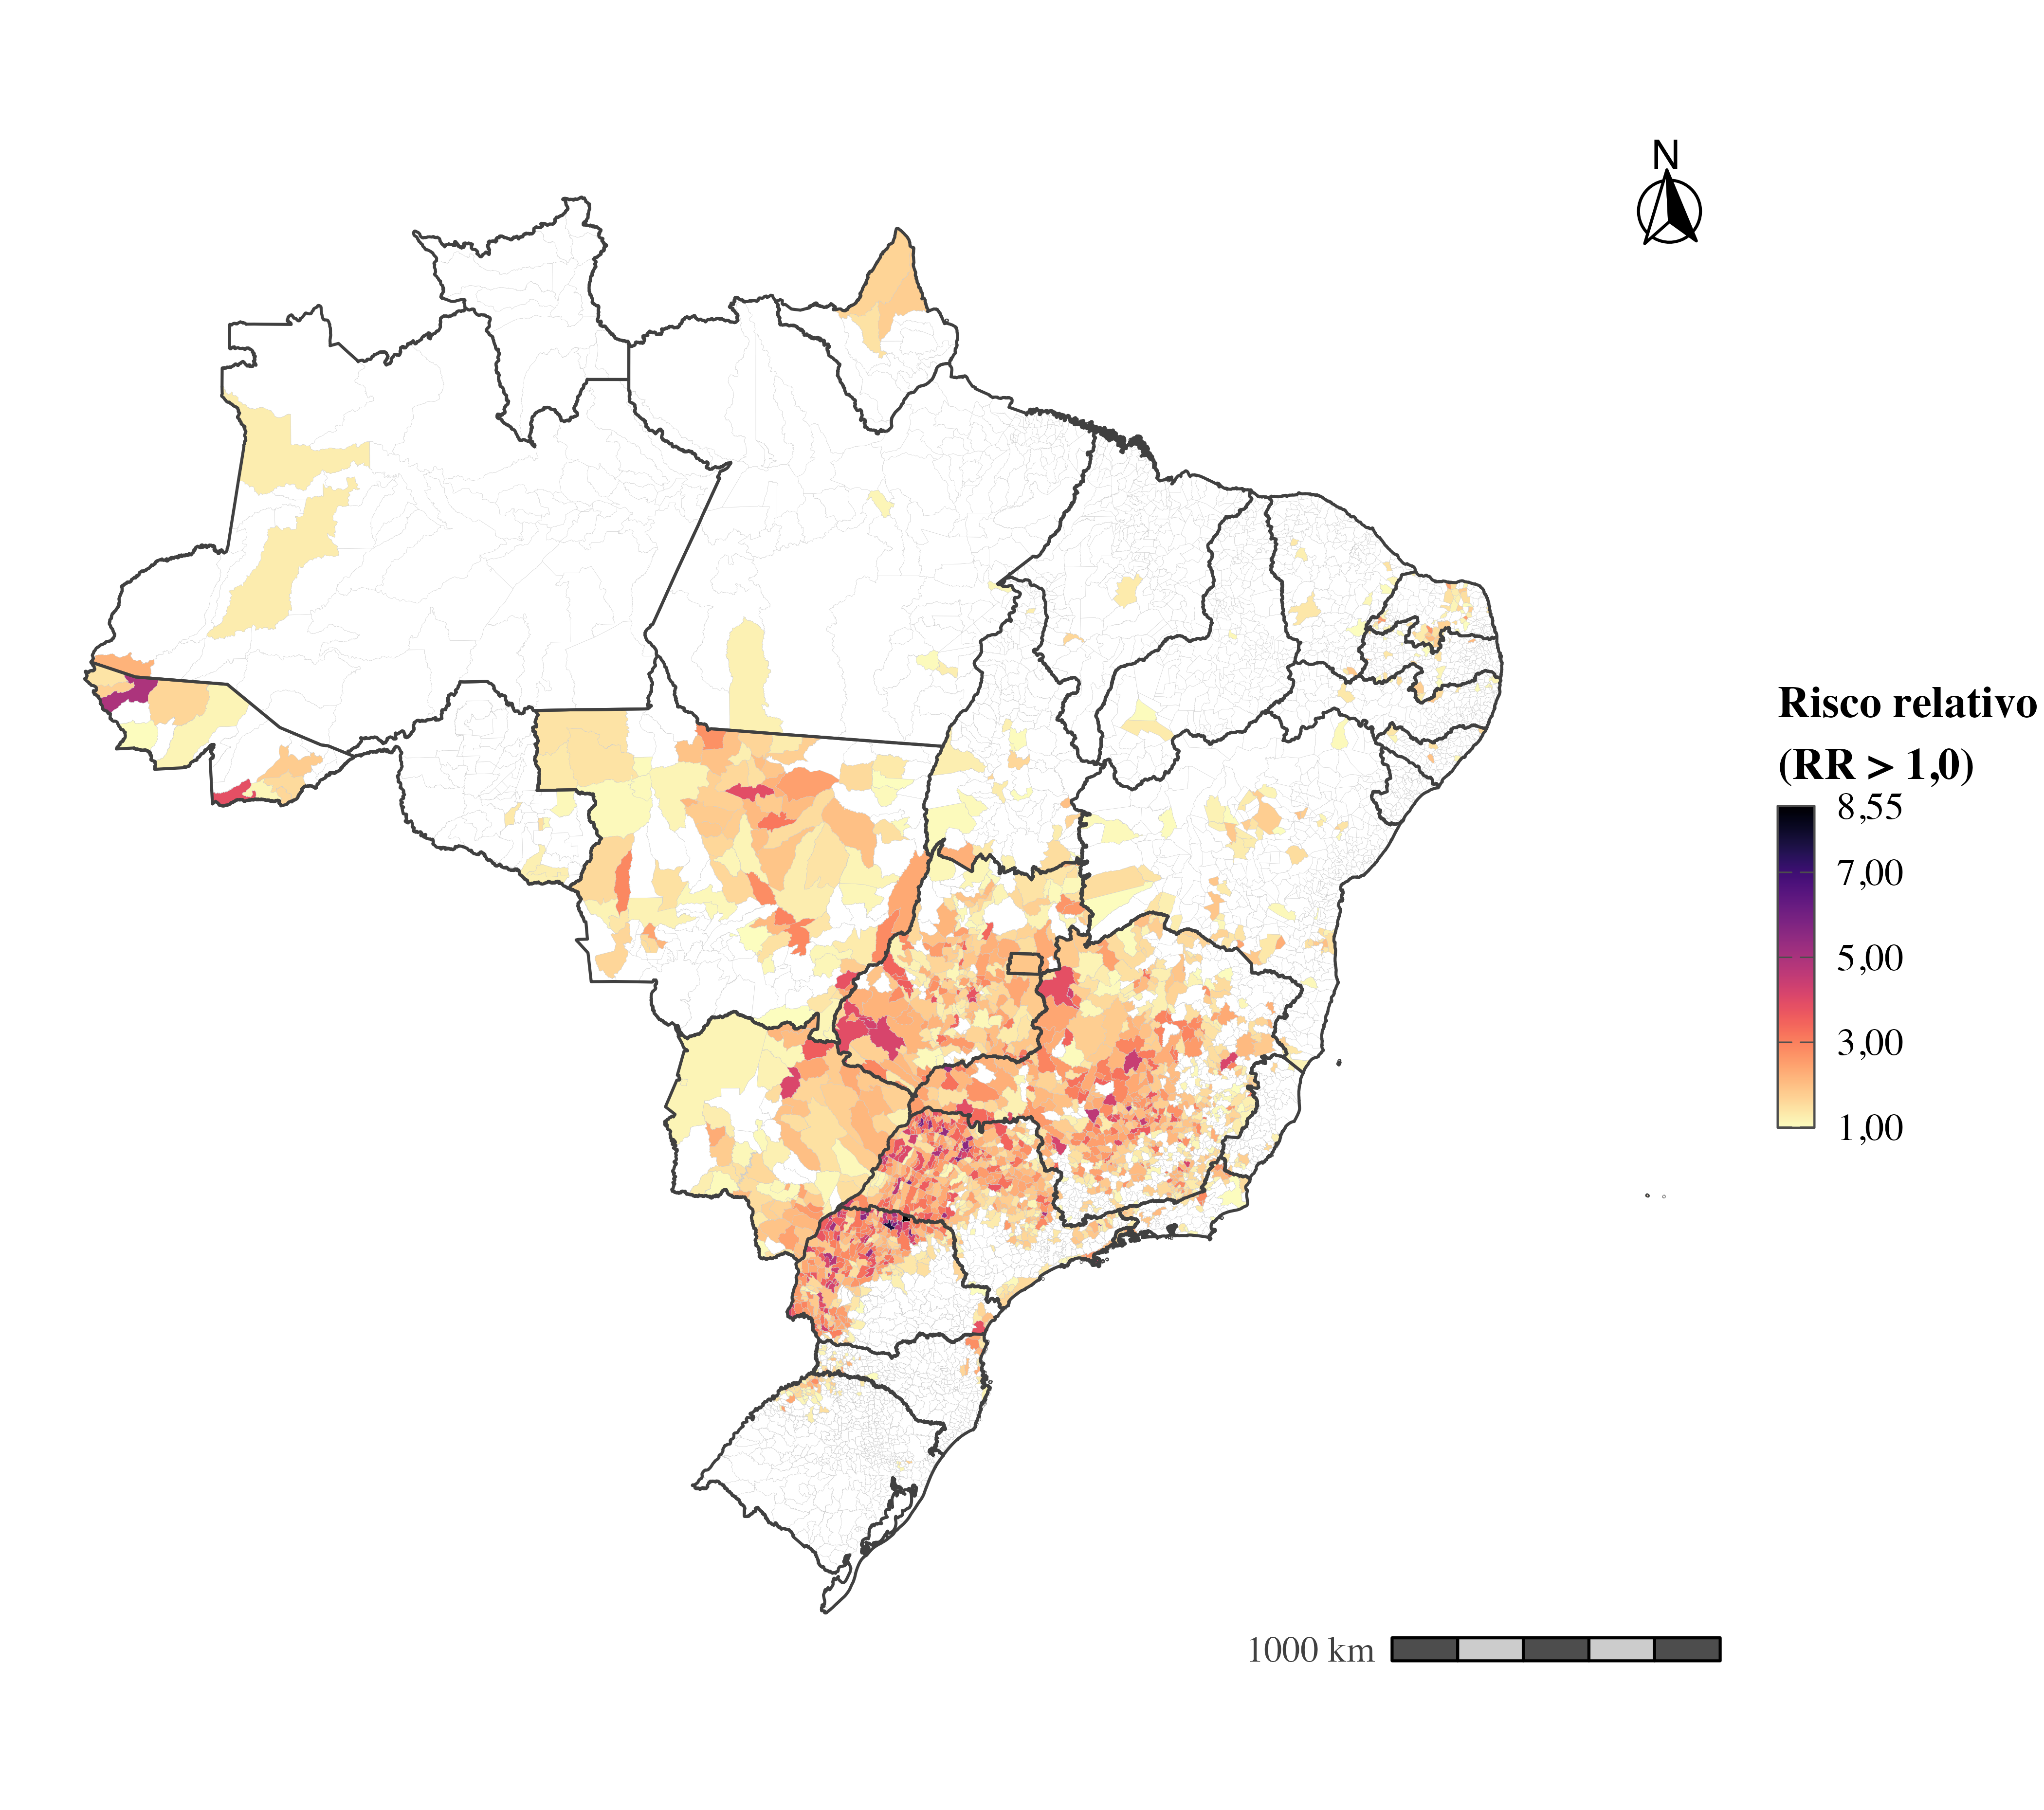
\includegraphics[width=\linewidth,height=6.15cm,keepaspectratio]{fig_mapa_rr_satscan_puro.png}
\end{column}\begin{column}{0.36\textwidth}Contraste municipal sob referência populacional homogênea.
\medskip
Tons mais escuros indicam RR mais alto.
\medskip
Branco: RR menor ou igual a 1.\end{column}\end{columns}\fonte{SINAN e IBGE; elaboração do autor.}
\note{Distinga o mapa de RR municipal do RR agregado de cada zona. Um município com RR alto pode não formar uma zona significativa sob as restrições de busca e reporte.}
\end{frame}

\begin{frame}{Risco relativo municipal sob calor}
\begin{columns}[c]\begin{column}{0.61\textwidth}\centering
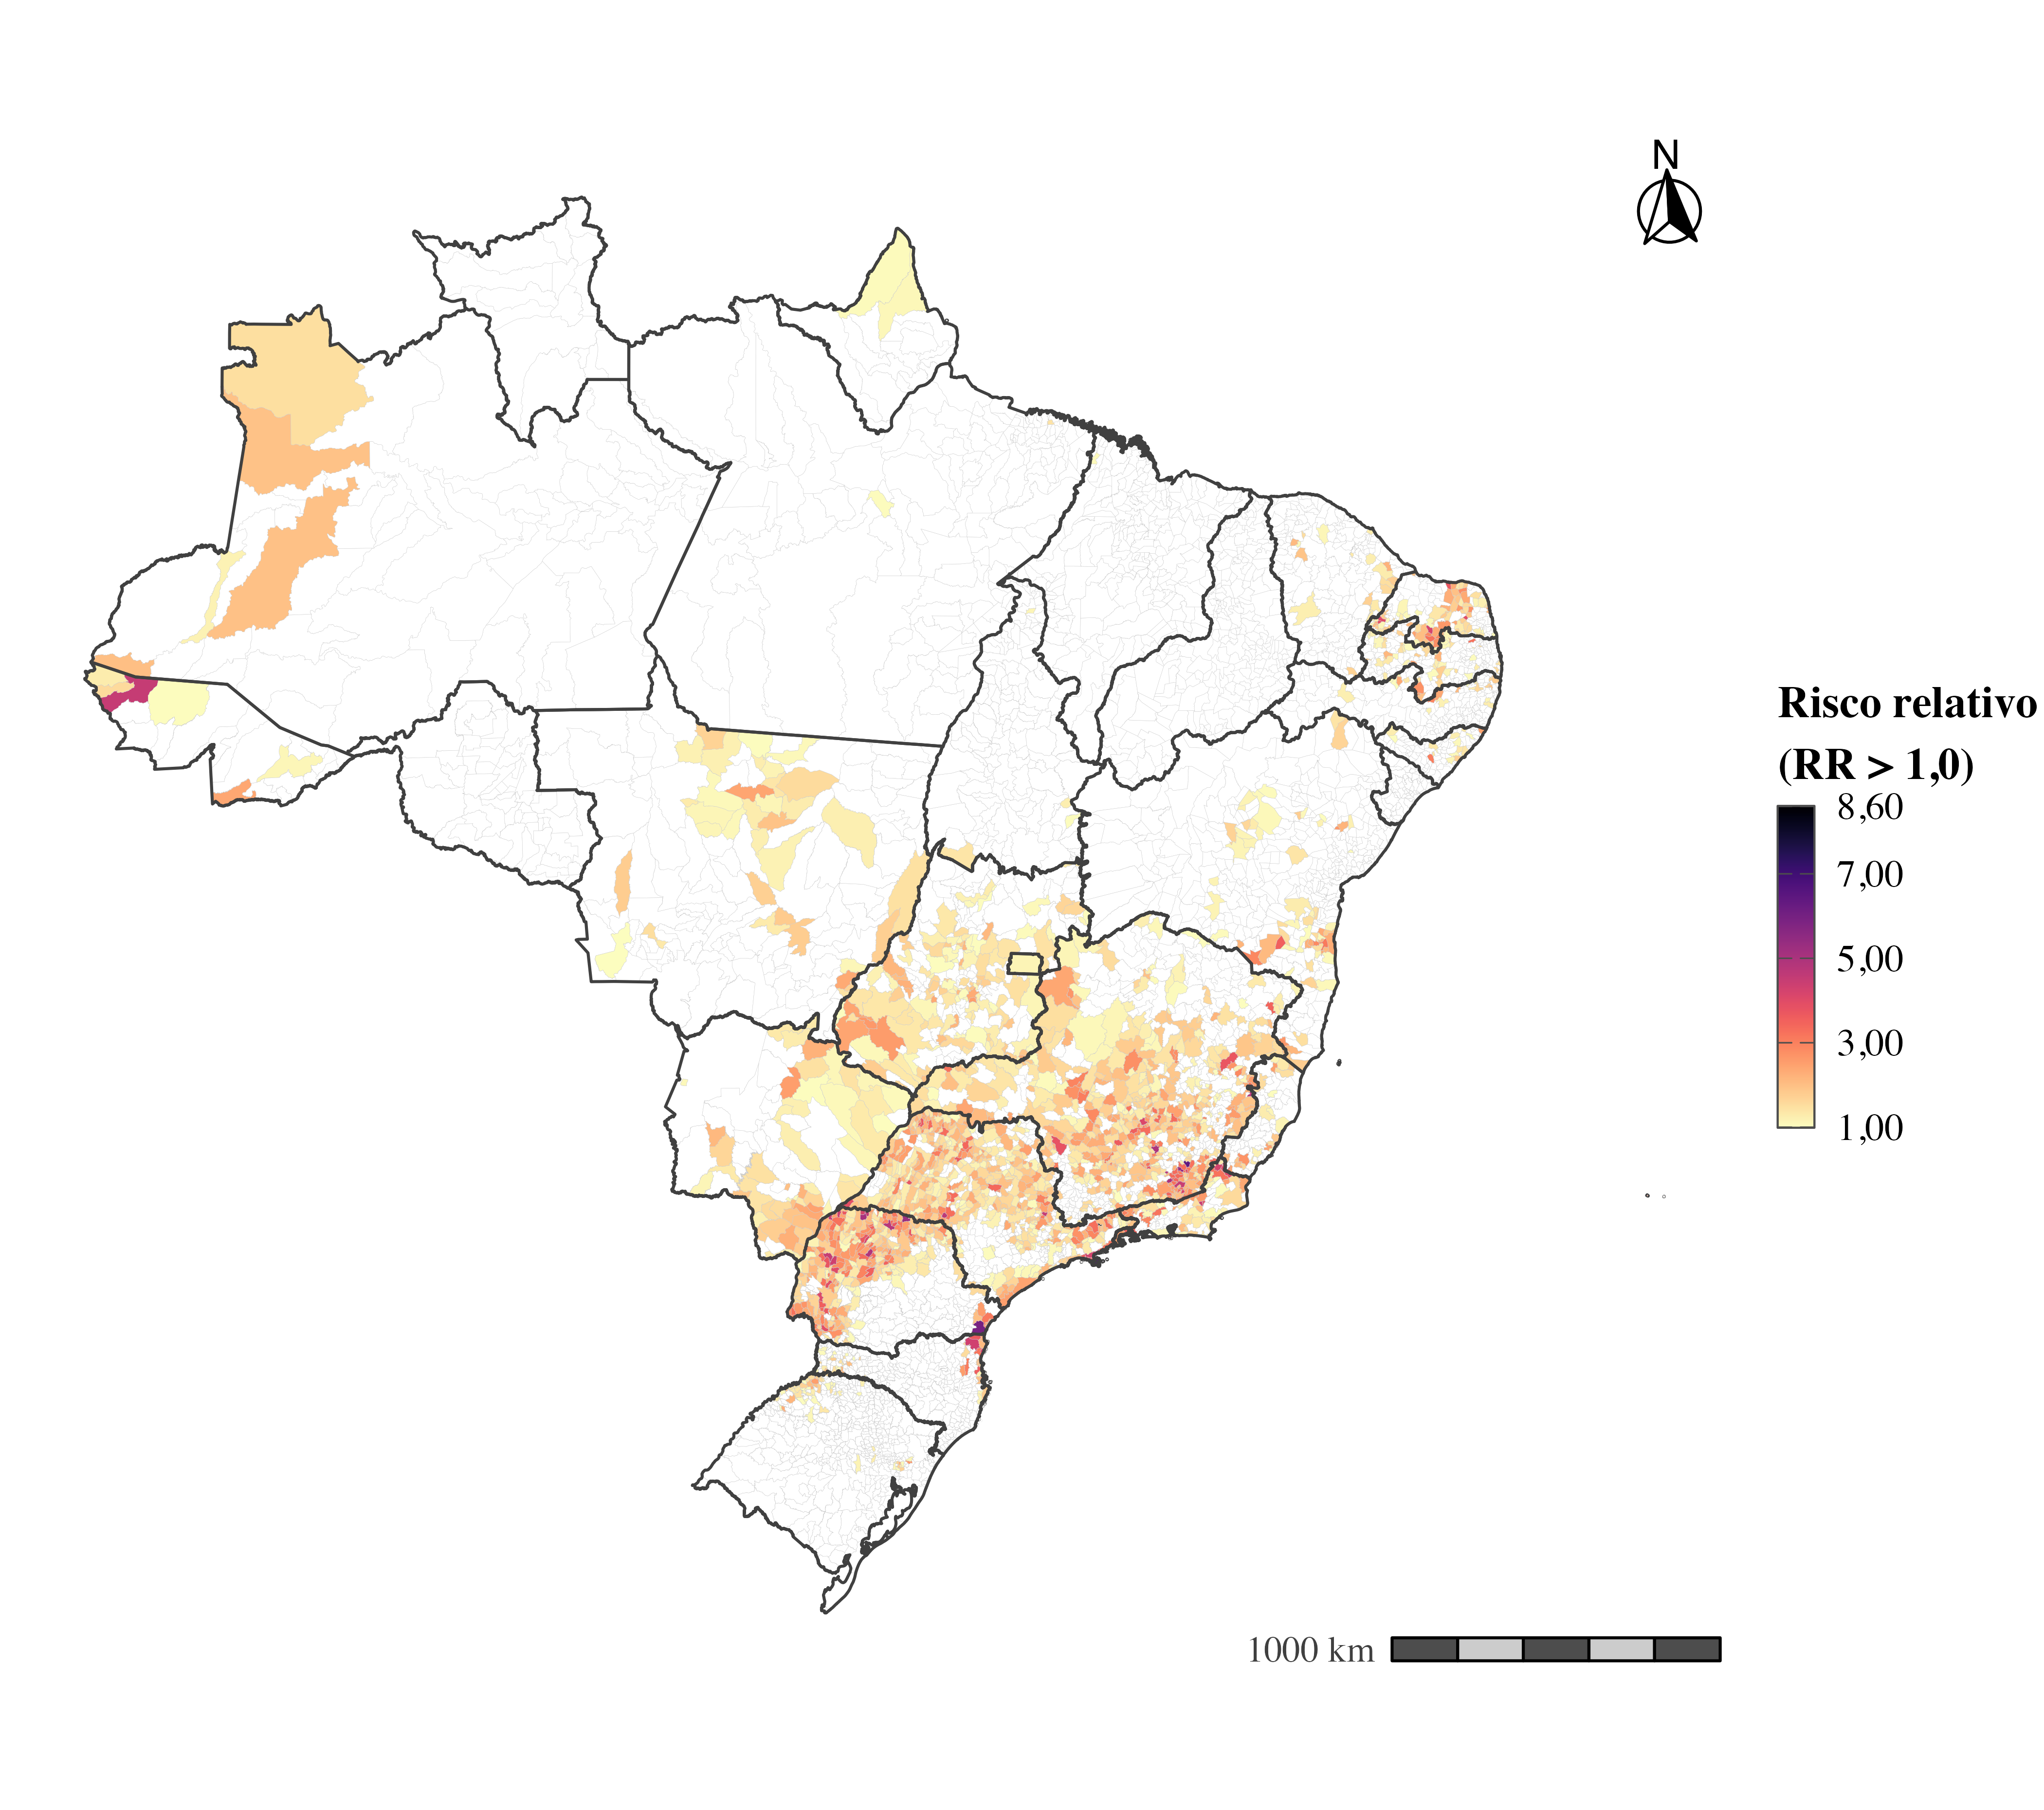
\includegraphics[width=\linewidth,height=6.15cm,keepaspectratio]{fig_mapa_rr_satscan_termica.png}
\end{column}\begin{column}{0.36\textwidth}A referência passa a considerar os tercis de dias de calor.
\medskip
Permanecem contrastes municipais após a padronização.
\medskip
\small Consulte os limites da legenda: estes mapas individuais têm escalas próprias.\end{column}\end{columns}\fonte{SINAN e IBGE; elaboração do autor.}
\note{Ao comparar mapas individuais, atenção aos limites das escalas. A comparação por intensidade deve usar números ou os painéis com escala comum do material de apoio. O ajuste descreve excesso residual, sem decompor causas.}
\end{frame}

\begin{frame}{WMAPE nacional e diferenças regionais}
\begin{tabularx}{\textwidth}{@{}Xrr@{}}\toprule
Região & Sem ajuste (\%) & Calor (\%)\\\midrule
Centro-Oeste &53,4&38,7\\
Sudeste &57,0&43,7\\
Sul &101,9&80,9\\
Nordeste &122,2&122,2\\
Norte &183,0&245,9\\\bottomrule
\end{tabularx}\par\vspace{0.25cm}\noindent O WMAPE nacional diminui, mas a proximidade ao observado não melhora em todas as regiões.\fonte{Decomposição regional do WMAPE; valores arredondados.}
\note{Valores regionais acima de 100\% são possíveis porque o esperado foi padronizado nacionalmente; ele não soma o observado dentro de cada região. O denominador regional pode ser pequeno em relação aos desvios acumulados. O resultado nacional dá maior peso às regiões com mais casos.}
\end{frame}

\begin{frame}{Recorrência entre as formulações}
\begin{columns}[c]\begin{column}{0.61\textwidth}\centering
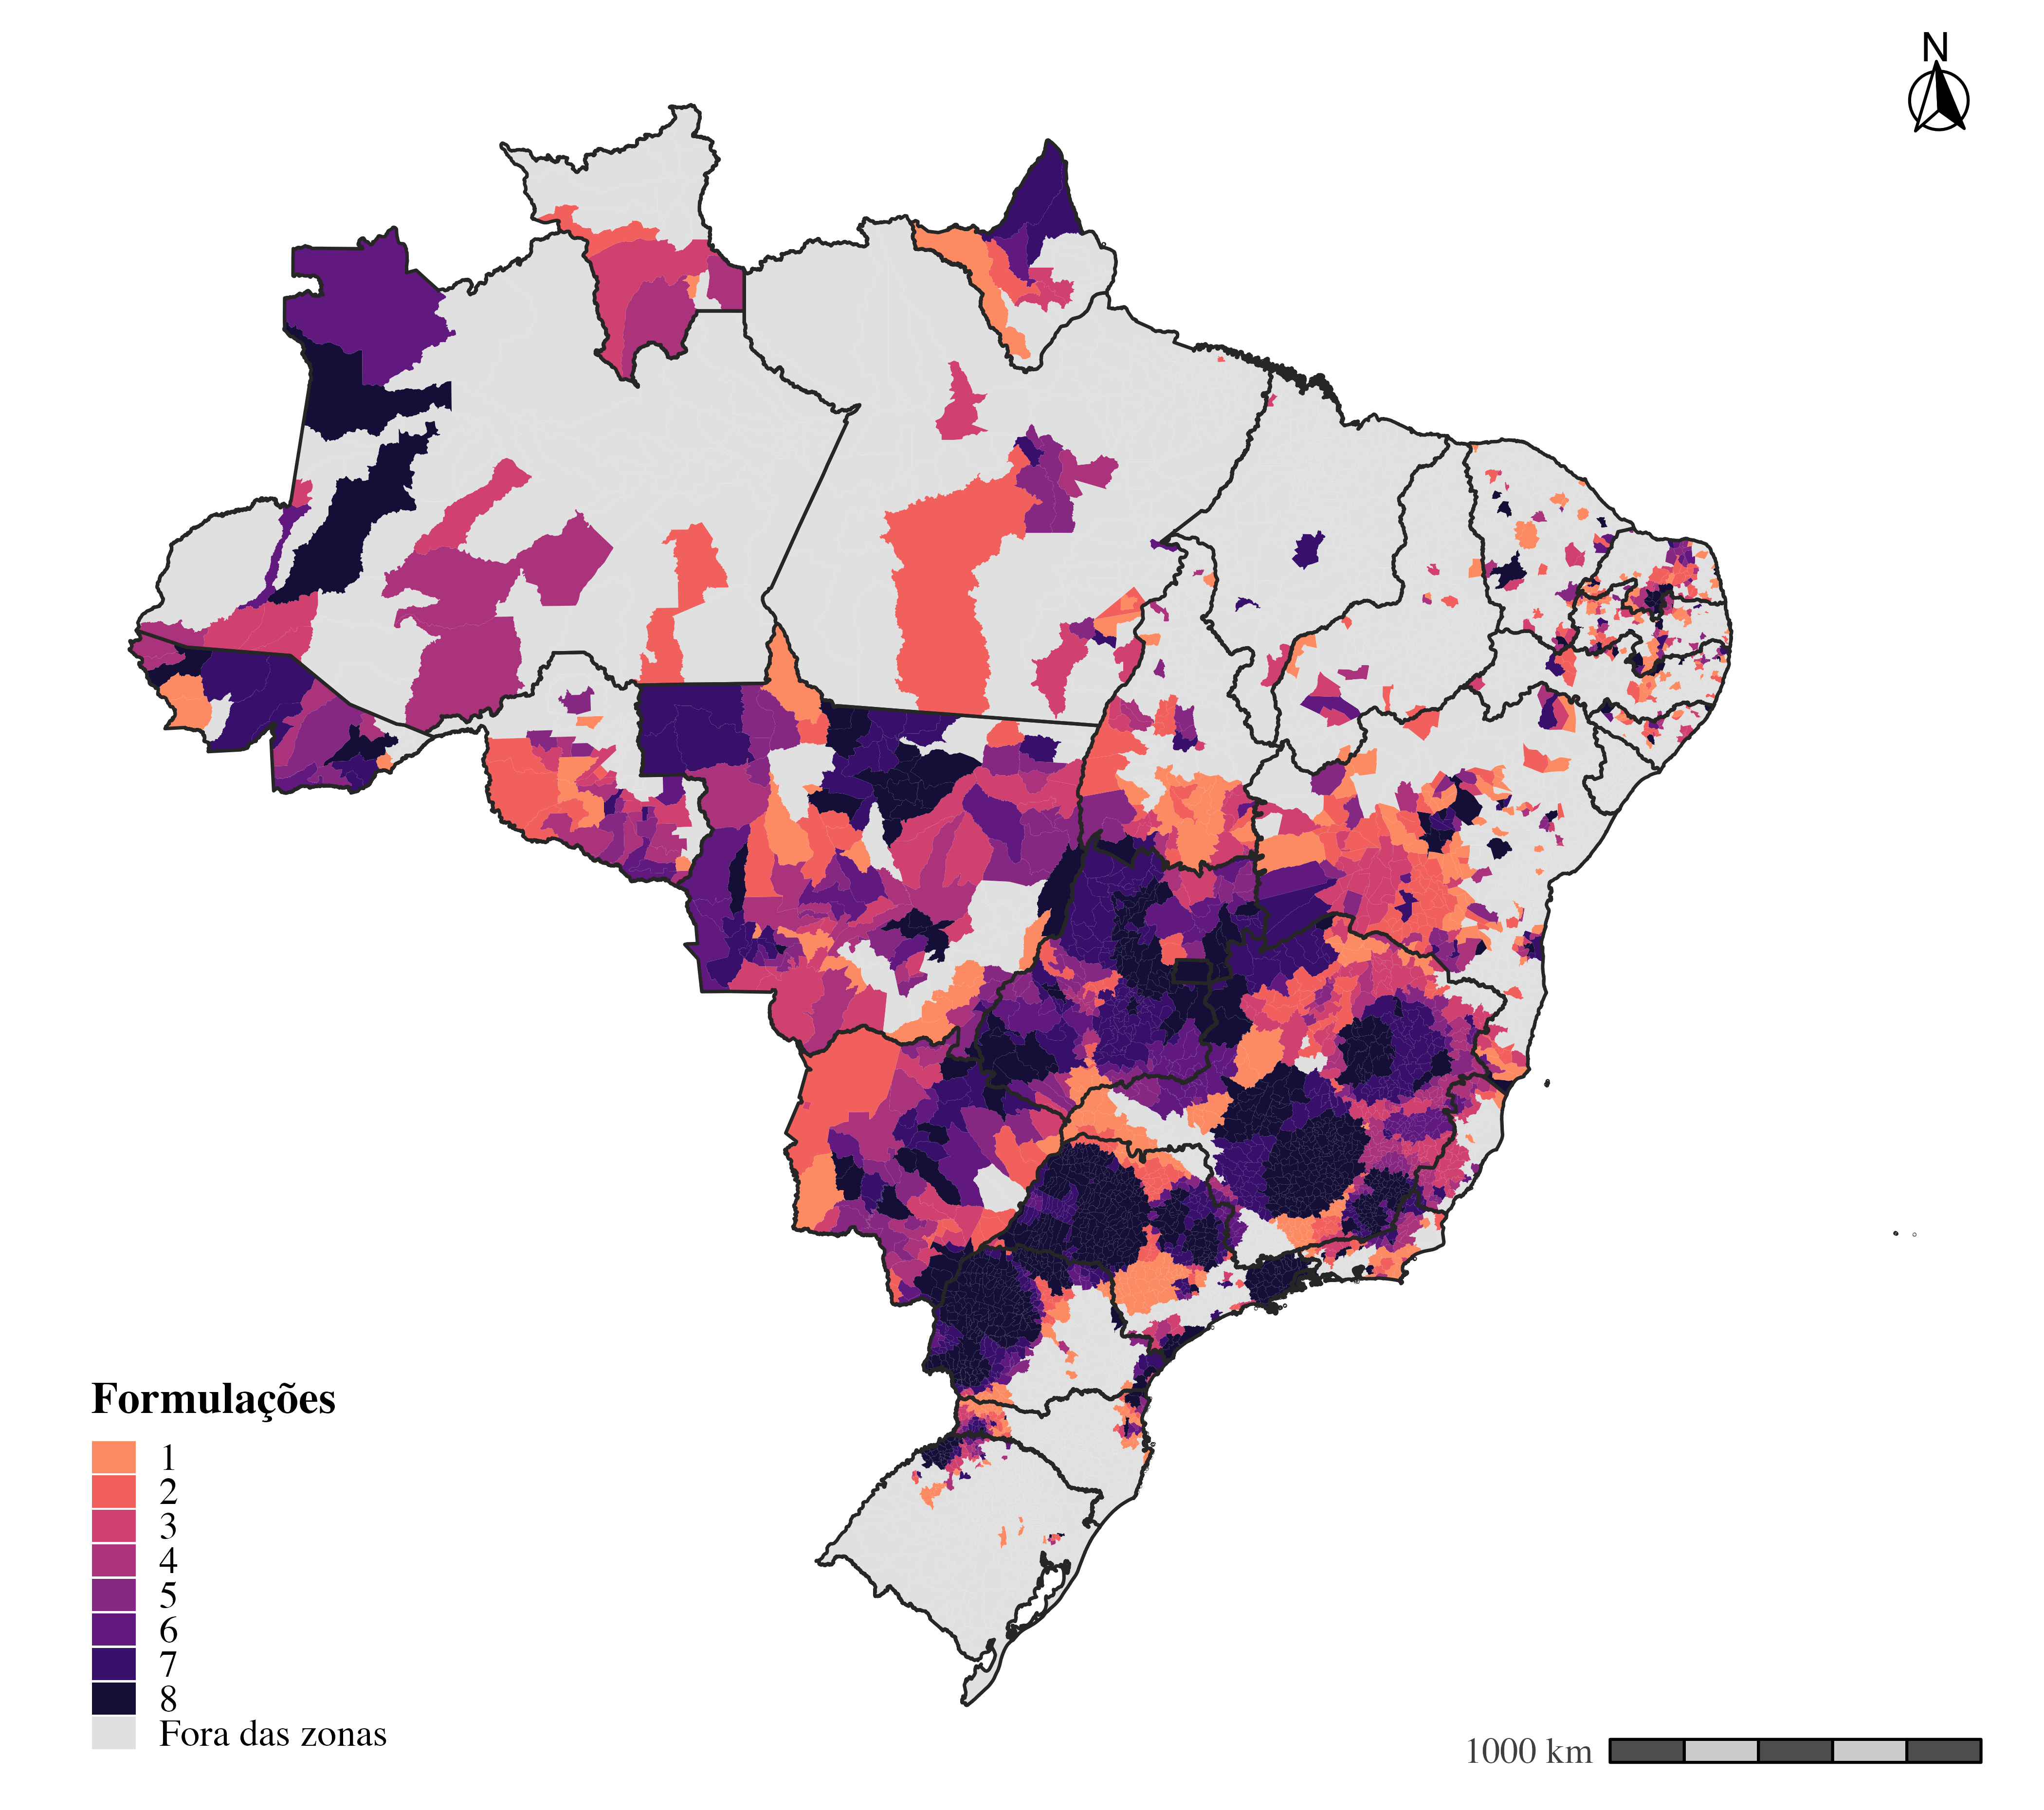
\includegraphics[width=\linewidth,height=6.15cm,keepaspectratio]{fig_mapa_persistencia_ajustes.png}
\end{column}\begin{column}{0.36\textwidth}3.016 municípios em pelo menos uma formulação.
\medskip
1.655 em seis ou mais.
\medskip
967 em todas as oito.
\medskip
\small Frequência de inclusão nas zonas; não mede intensidade do excesso.\end{column}\end{columns}\fonte{SINAN e IBGE; elaboração do autor.}
\note{A contagem pesa igualmente as oito formulações, que não são independentes. Não é uma probabilidade de risco nem uma frequência em anos. Evite confundir esta recorrência entre modelos com persistência epidêmica temporal.}
\end{frame}

\begin{frame}{Sensibilidade à exclusão de 2024}
\small\begin{tabularx}{\textwidth}{@{}Xrrr@{}}\toprule
Formulação & Com 2024 & Sem 2024 & Jaccard (\%)\\\midrule
Sem ajuste&129&169&61\\
Calor&128&130&51\\
Esgoto&178&174&63\\
Densidade urbana&136&168&55\\
Proporção urbana&158&173&58\\
Água&193&188&60\\
Lixo&195&186&60\\
Índice composto&184&196&61\\\bottomrule
\end{tabularx}\par\vspace{0.25cm}\noindent\normalsize A contagem muda em todas as formulações; o polo primário muda em sete.
%\fonte{Consolidação dos cenários. Colunas centrais: número de zonas.}
\note{Mesmo aumentando o número de zonas em parte dos modelos, a retirada de 2024 não amplia necessariamente a mesma coleção municipal. Jaccard descreve o quanto ela se mantém.}
\end{frame}

\begin{frame}{Zonas sem ajuste no cenário sem 2024}
\begin{columns}[c]\begin{column}{0.61\textwidth}\centering
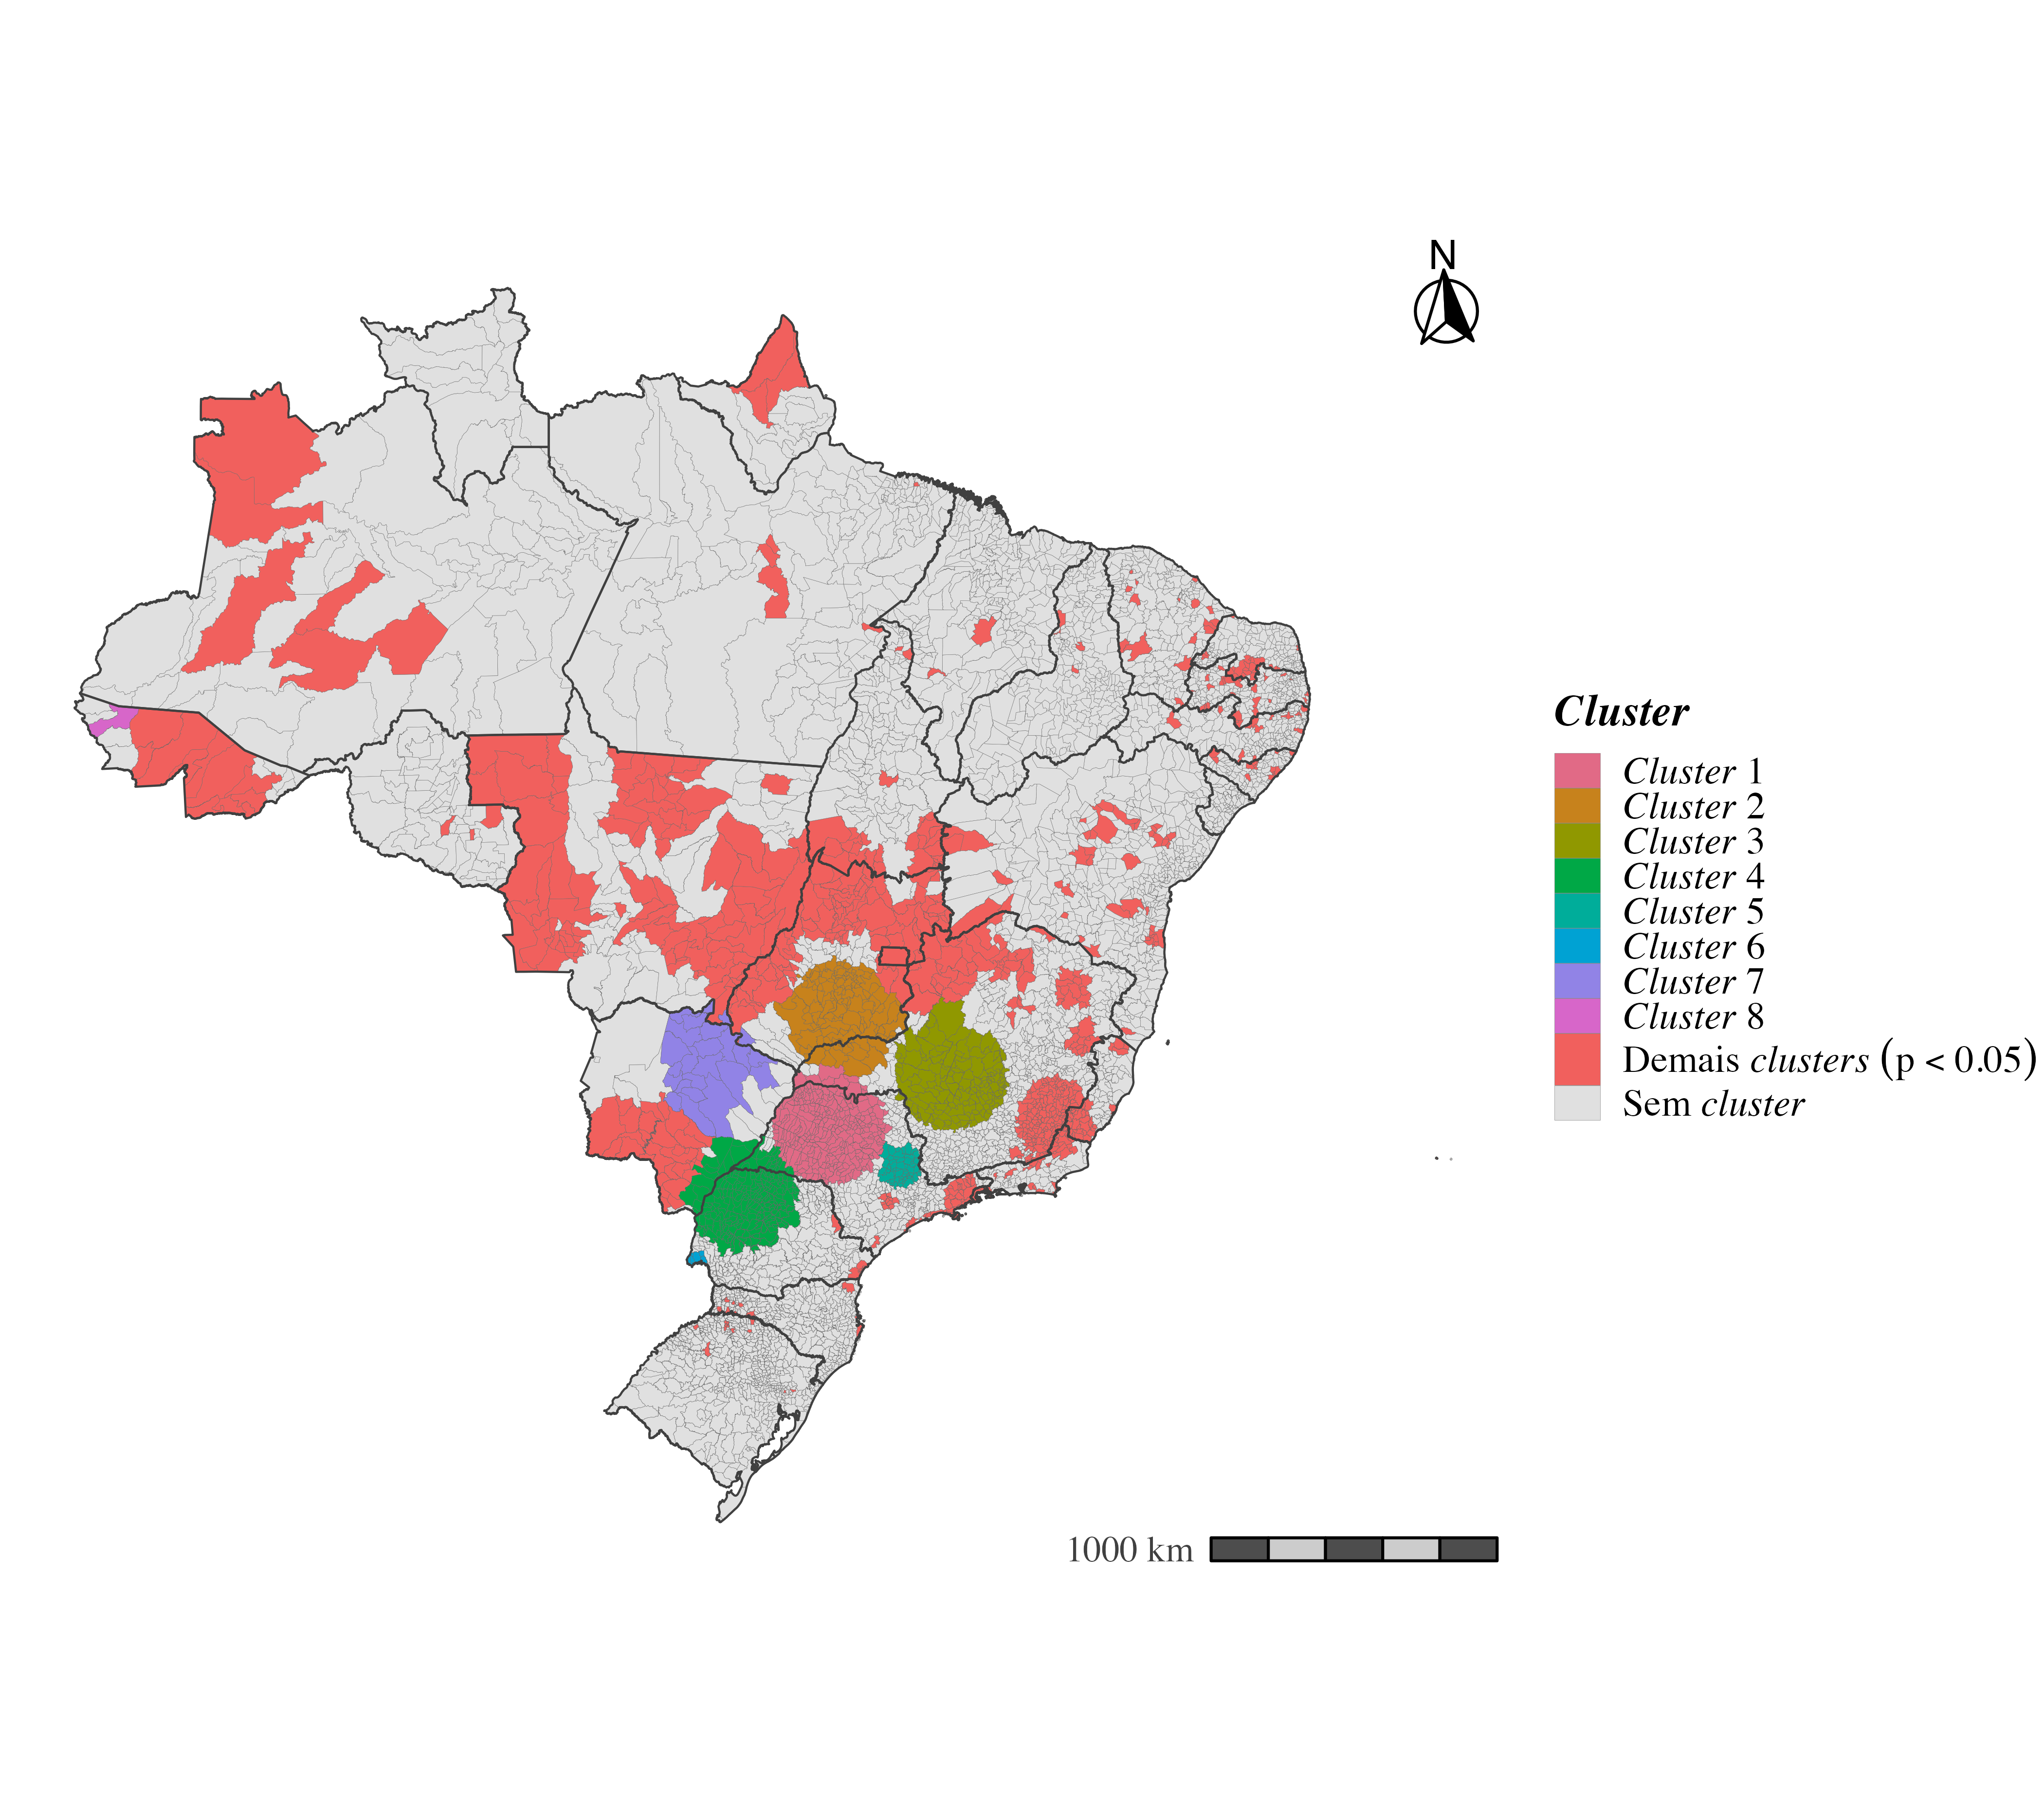
\includegraphics[width=\linewidth,height=6.15cm,keepaspectratio]{fig_mapa_clusters_satscan_puro_sem2024.png}
\end{column}\begin{column}{0.36\textwidth}169 zonas; polo primário em Ubarana (SP).\par\medskip Sobreposição municipal de 61\% com a coleção do período completo.\par\medskip A mudança envolve a composição das zonas, além de sua contagem.\end{column}\end{columns}\fonte{SINAN e IBGE; elaboração do autor.}
\note{Compare com o mapa sem ajuste apresentado anteriormente. O cenário mantém 2010 a 2023 e 2025. O aumento no número de zonas não significa aumento do total de casos.}
\end{frame}

\section{Discussão e encerramento}
\begin{frame}{Interpretação dos achados}
\begin{itemize}
\item A autocorrelação anual e as zonas acumuladas descrevem uma distribuição espacial estruturada.
\item A concentração no Centro-Sul reaparece sob referências distintas; os limites e os polos das zonas variam.
\item A padronização por calor reduz mais o WMAPE nacional, com piora no Norte.
\item O peso de 2024 altera a leitura acumulada e deve acompanhar a interpretação dos mapas.
\end{itemize}\fonte{Diálogo com \cite{lee2021,lowe2021}; comparações exploratórias.}
\note{Separe o observado das hipóteses. Clima, infraestrutura e conectividade podem ser discutidos à luz da literatura, mas não foram isolados causalmente. As análises descrevem notificações e referências de excesso, não mecanismos individuais de infecção.}
\end{frame}

\begin{frame}{Limitações}
\begin{itemize}
\item Subnotificação, atrasos e diferenças de vigilância entre municípios.
\item Agregação municipal, resolução climática e saneamento fixo em 2022.
\item Restrição circular, limites da janela e hipótese de Poisson.
\item Testes locais e reporte secundário exploratórios; significância pode acompanhar excessos pequenos em bases grandes.
\item WMAPE interno à amostra e covariáveis categorizadas; ausência de inferência causal.
\end{itemize}
\note{A unidade ecológica impede extrapolar associações municipais para indivíduos. A varredura acumulada não informa quando cada zona surgiu. A contagem de inclusão entre modelos não pondera intensidade. Esses limites orientam as conclusões, sem invalidar a descrição produzida.}
\end{frame}

\begin{frame}{Considerações finais}
\begin{itemize}
\item A incidência apresenta associação espacial positiva nos 16 anos.
\item A varredura delimita zonas de excesso de notificações, sobretudo no Centro-Sul.
\item A referência dos esperados e o período analisado alteram a composição dessas zonas.
\item O estudo oferece uma descrição territorial comparável e explicita a sensibilidade das escolhas analíticas.
\end{itemize}
\note{Encerre respondendo aos objetivos. Como continuação, proponha modelos ecológicos explícitos, avaliação fora da amostra quando houver finalidade preditiva e janelas flexíveis. Abra para as perguntas da banca sem introduzir um novo resultado.}
\end{frame}

\appendix
\section{Apoio}
\begin{frame}{Comparação do RR em escala comum}
\centering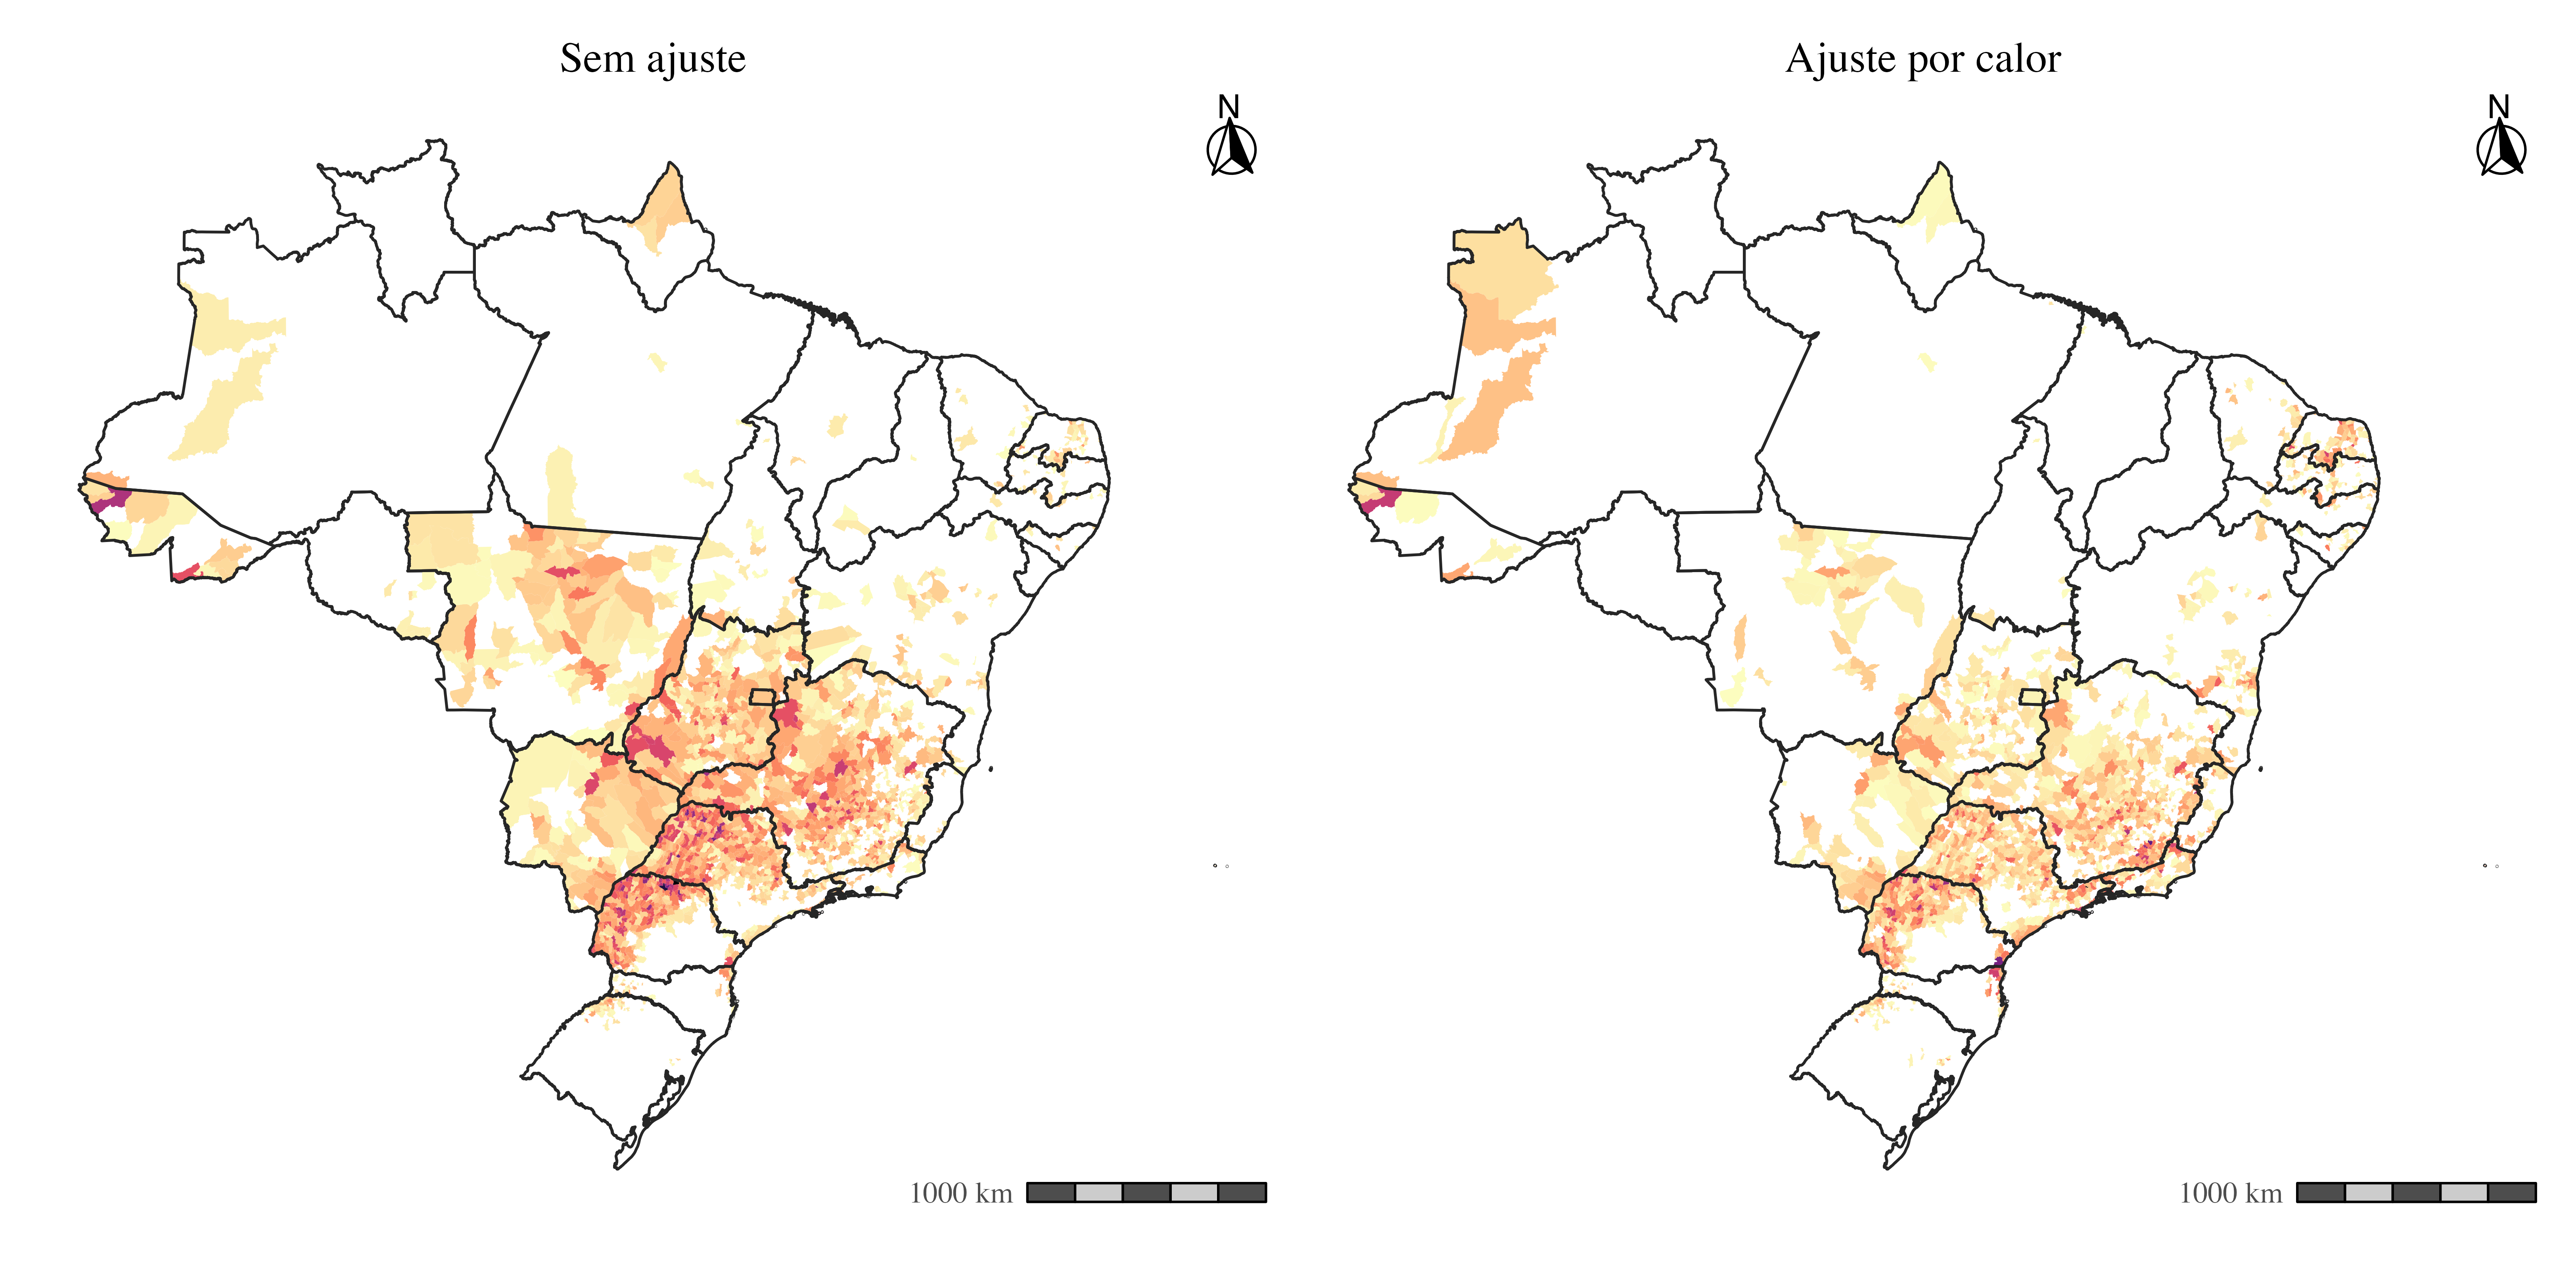
\includegraphics[width=0.95\textwidth,height=4.9cm,keepaspectratio]{fig_slides_rr_puro_calor.png}\par\vspace{0.05cm}
\includegraphics[width=0.95\textwidth,height=0.9cm,keepaspectratio]{legenda_rr_slides_puro_calor.pdf}\fonte{Branco: $RR\leq1$. Fontes: SINAN e IBGE; elaboração do autor.}
\note{Use para comparar cores entre as duas referências. A legenda numérica tem os mesmos limites e a mesma paleta nos dois mapas. A comparação municipal é distinta da comparação dos dois primários, que têm composições diferentes.}
\end{frame}

\section{Referências}
\begin{frame}[allowframebreaks]{Referências citadas}
\scriptsize\bibliography{../tex/referencias}
\end{frame}
\end{document}
